\documentclass{beamer}
\usepackage[spanish]{babel}
\usepackage[utf8]{inputenc}
\usepackage{multicol} % indice en 2 columnas
\usepackage{centernot}
\usepackage{amsmath}% http://ctan.org/pkg/amsmath

\usepackage{color}


\usepackage{graphicx}
\graphicspath{ {im/} }


\newcommand{\notimplies}{%
  \mathrel{{\ooalign{\hidewidth$\not\phantom{=}$\hidewidth\cr$\implies$}}}}


\usetheme{Warsaw}
%\usecolortheme{crane}
\useoutertheme{shadow}
\useinnertheme{rectangles}

\setbeamertemplate{navigation symbols}{} % quitar simbolitos



\title[Tema 8 - Introducció a la Teoria de Grafs]{Teoria de grafs}
\subtitle{Grau en Enginyeria Telemàtica}
\author[Juan Gabriel Gomila]{
Juan Gabriel Gomila%$^{1}$  \and E. Eva$^{2}$ \and S. Serpiente$^{3}$
}
\institute[UIB]{
 % $^{1-2}$
 Grau en Enginyeria Telemàtica
 \and
  Universitat de les Illes Balears
  \and
  \texttt{juangabriel.gomila@uib.es}
}
\date{\today}

\AtBeginSection{
\begin{frame}
  \begin{multicols}{2}
  \tableofcontents[currentsection]   
\end{multicols}
\end{frame}
}

\AtBeginSubsection{
\begin{frame}
  \begin{multicols}{2}
  \tableofcontents[currentsection,currentsubsection]
\end{multicols}
\end{frame}
}



%empieza aqui


\begin{document} 

\frame{\titlepage}

\begin{frame}
  \frametitle{Índex}
  \tableofcontents
\end{frame}

\section{Teoria de Grafs}
\subsection{Una mica d'historia}


\begin{frame}
\frametitle{D'on venen els grafs}
La teoria de grafs és una branca de la matemàtica que ha sorgit i s'ha desenvolupat per donar solucions a problemes molt concrets. 

El problema que la majoria d'autors assenyalen com a l'origen de la teoria de grafs és el \textbf{problema dels ponts de Königsberg}


\begin{figure}[h]
 \label{fig:volum}
\centering
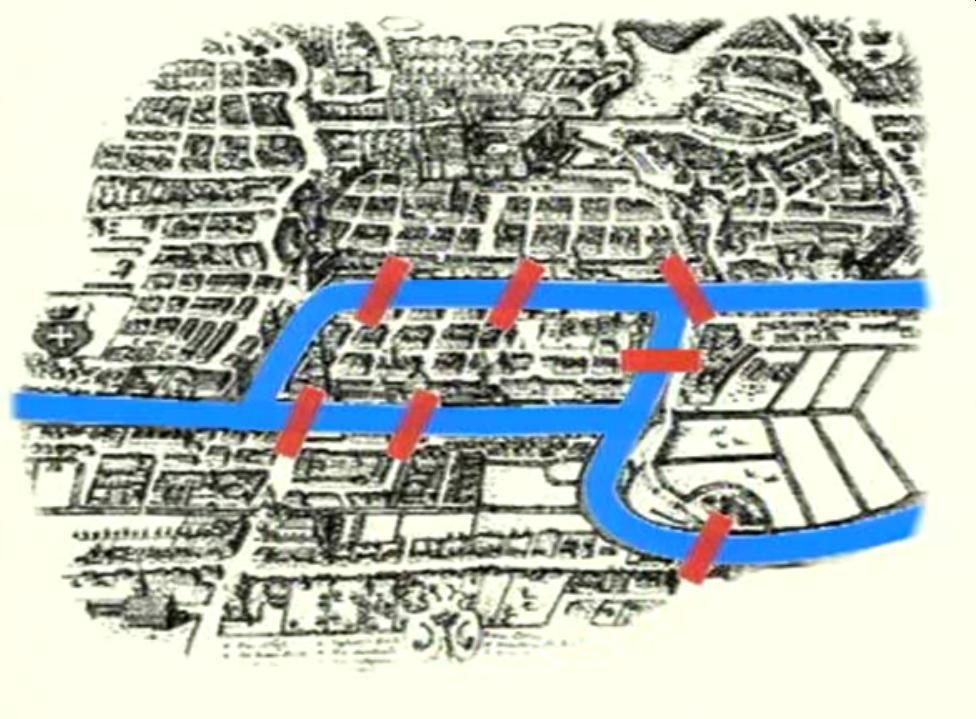
\includegraphics[height=5cm]{konisgberg}
\end{figure}
 
\end{frame}

\begin{frame}
\frametitle{D'on venen els grafs}
Durant el segle XVIII, la ciutat de Künigsberg (la Prúsia Oriental( estava dividida en quatre zones pel riu Prevel. Hi havia set punts que comunicaven aquestes regions com demostra el dibuix.

\begin{figure}[h]
 \label{fig:volum}
\centering
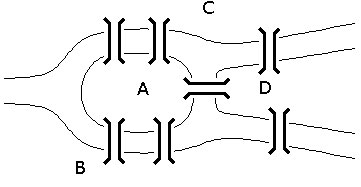
\includegraphics[height=5cm]{kon2}
\end{figure}
\end{frame}


\begin{frame}
\frametitle{D'on venen els grafs}
Els habitants de la ciutat no tenien biofestes ni univerlands, i enlloc de tenir les mateixes necessitats que vosaldres, volien trobar, si era possible una manera de passejar per la ciutat que els permetès anar d'una determinada regio, creuar cada pont una única vegada i tornar al lloc de partida. 
\begin{figure}[h]
 \label{fig:volum}
\centering

\includegraphics[height=4.8cm]{univerland}
\end{figure}
\end{frame}


\begin{frame}
\frametitle{D'on venen els grafs}
Per a resoldre aquest problema, Euler va representar les quadre zones de la ciutat per quatre punts i els ponts per arestes que uneixen els punts, tal i com es veu a la figura
\begin{figure}[h]
 \label{fig:volum}
\centering
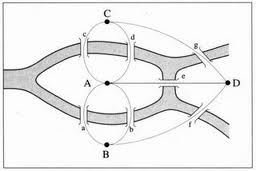
\includegraphics[height=4.8cm]{kon3}
\end{figure}
\end{frame}


\begin{frame}
\frametitle{D'on venen els grafs}
Actualment, la teoria de grafs s'aplica dins i fora de les matemàtiques i segueix sent una branca d'investigació molt activa. Les seves aplicacions són molt importants a l'enginyeria i resulten de gran utilitat per a la representació de dades, disseny de xarxes de telecomunicació...
\end{frame}

\subsection{Per què me pot servir un graf?}

\begin{frame}
\frametitle{Els xuts de la selecció}
\begin{figure}[h]
 \label{fig:volum}
\centering
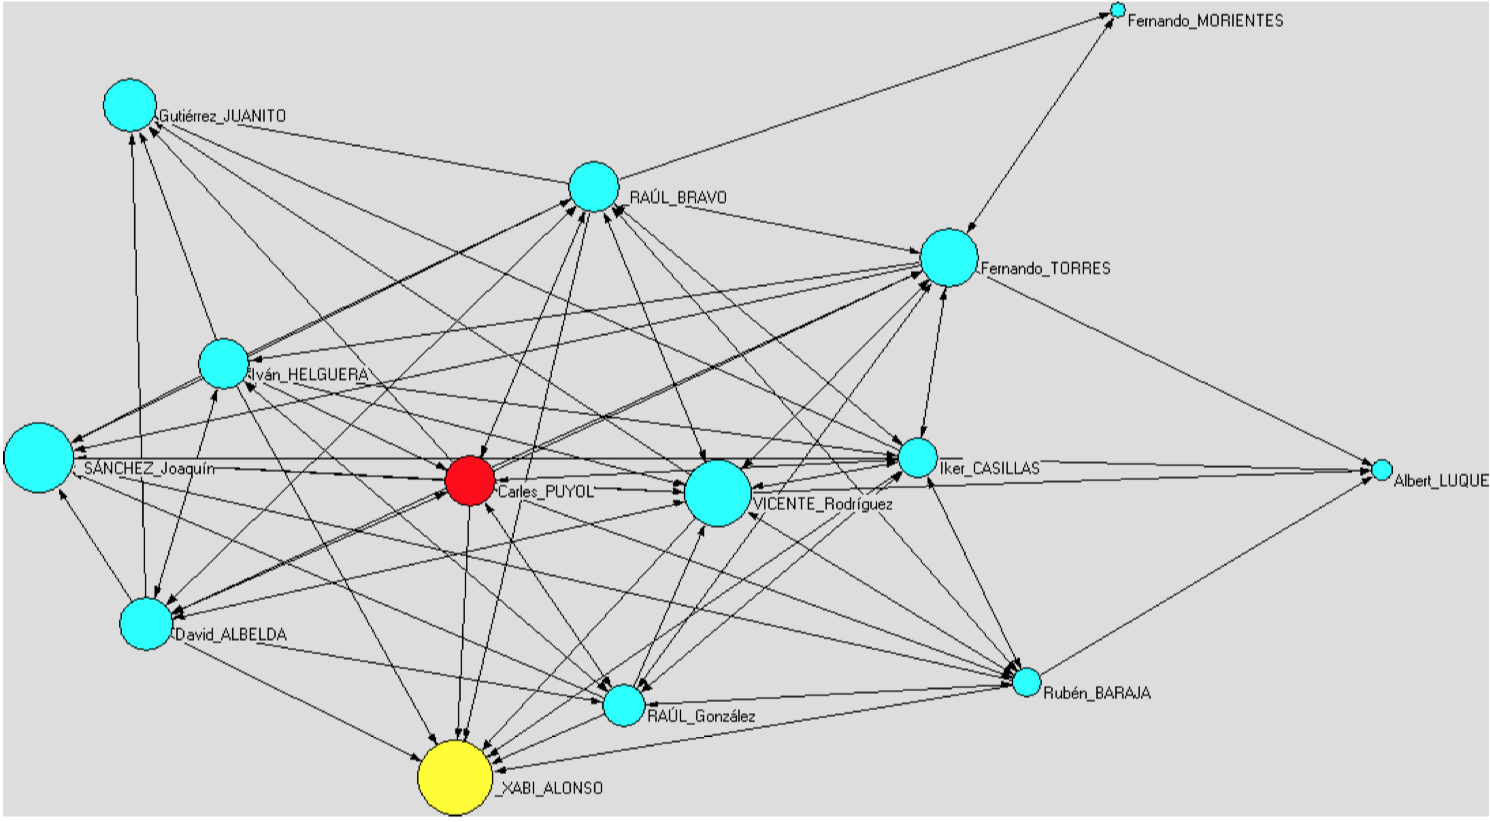
\includegraphics[height=5.5cm]{futbol1}
\end{figure}
Per saber les relacions entre passades i xuts dels jugadors de la selecció espanyola en el partit Espanya - Portugal del 2004
\end{frame}

\begin{frame}
\frametitle{Relacions sexuals a Anatomia de Grey}
Per representar totes les relacions sexuals a Anatomia de Grey i preveure quines hi haurà a les pròximes temporades (spoiler!)

\begin{figure}[h]
 \label{fig:volum}
\centering
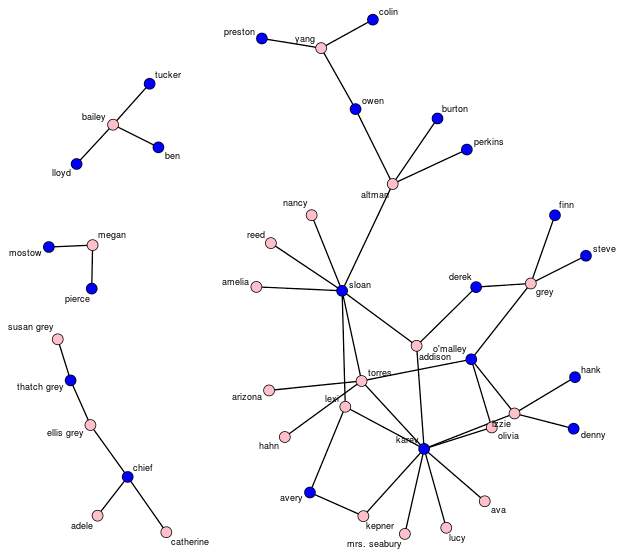
\includegraphics[height=6cm]{grey1}
\end{figure}
\end{frame}




\begin{frame}
\begin{figure}[h]
 \label{fig:volum}
\centering
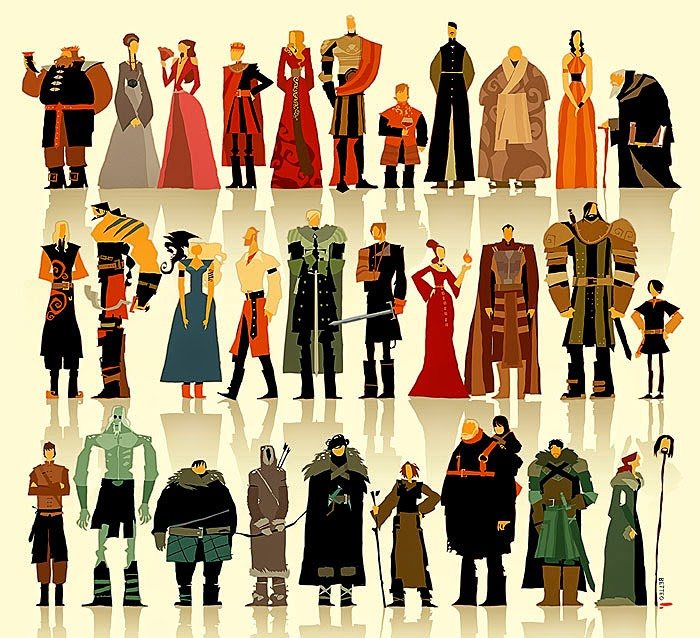
\includegraphics[height=8cm]{got1}
\end{figure}
\end{frame}

\begin{frame}
\frametitle{Relacions entre personatges de Game of Thrones}
Per representar les relacions i relevància dels personatges de GoT (en particular del llibre Storm of Swords)

\begin{figure}[h]
 \label{fig:volum}
\centering
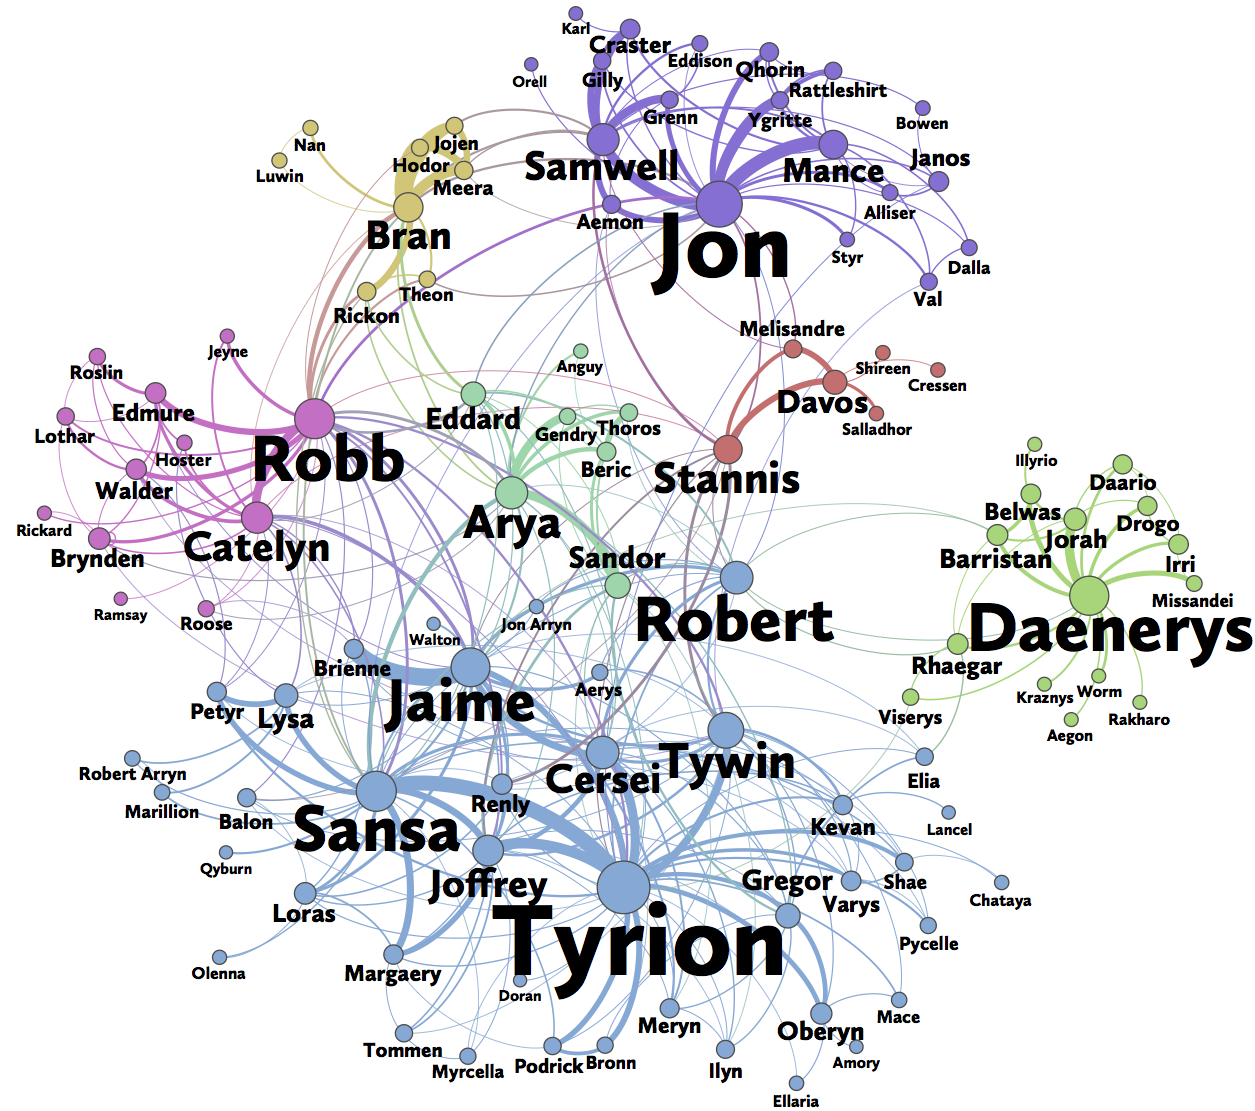
\includegraphics[height=6cm]{got2}
\end{figure}
\end{frame}

\section{El concepte de graf}


\begin{frame}
\frametitle{Què és un graf?}
Els grafs poden ser considerats formalment com a diagrames (representacions geomètriques) o bé algebraicament com un parell de conjunts (representacions algebraiques). Vegem ambdós tipus de definicions.
\end{frame}

\subsection{Definició geomètrica de graf}
\begin{frame}
\frametitle{Definició geomètrica de graf}
\begin{block}{Definició}
Geomètricament, un graf $G$ és un conjunt de punts a l'espai, alguns dels quals estan units entre ells mitjançant línies. 
\end{block}
Aquest graf pot simbolitzar per exemple un mapa de carreteres on els punts representen cuitats i les línies representen les carreteres que les uneixen. En aquest cas, el graf ens pot informar de les possibles comunicacions que existeixen entre les ciutats, però també aquest graf $G$ podria esquematitzar un circuït elèctric. 

\begin{figure}[h]
 \label{fig:volum}
\centering
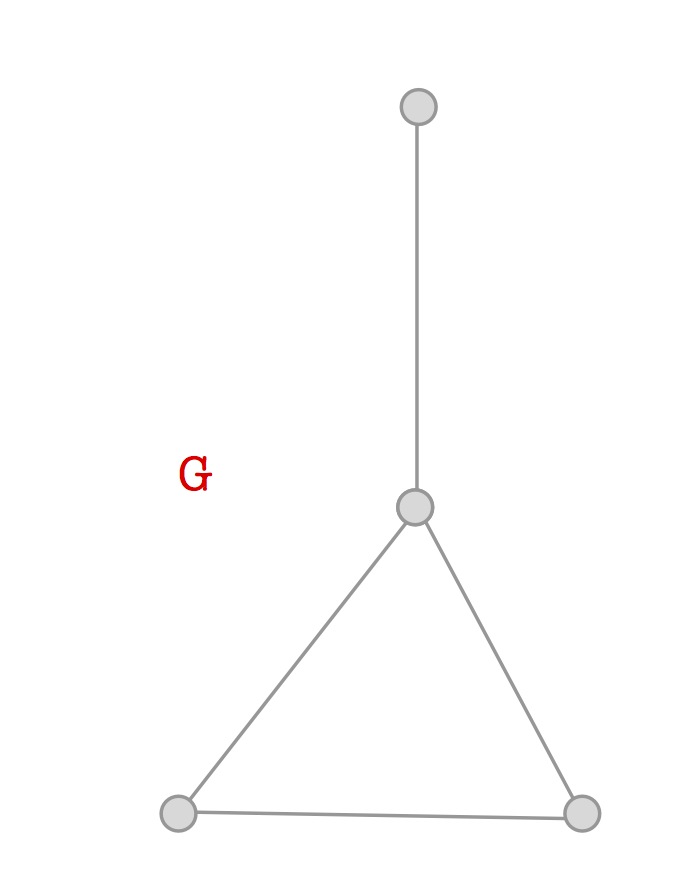
\includegraphics[height=3cm]{g1}
\end{figure}\end{frame}





\begin{frame}
\frametitle{Definició geomètrica de graf}

Hem de fer notar que un graf només conté informació sobre la connectivitat entre punts i no dóna informació geomètrica en sentit euclidià (distàncies, àngles...) Així els següents diagrames representen el mateix graf. 


\begin{figure}[h]
 \label{fig:volum}
\centering
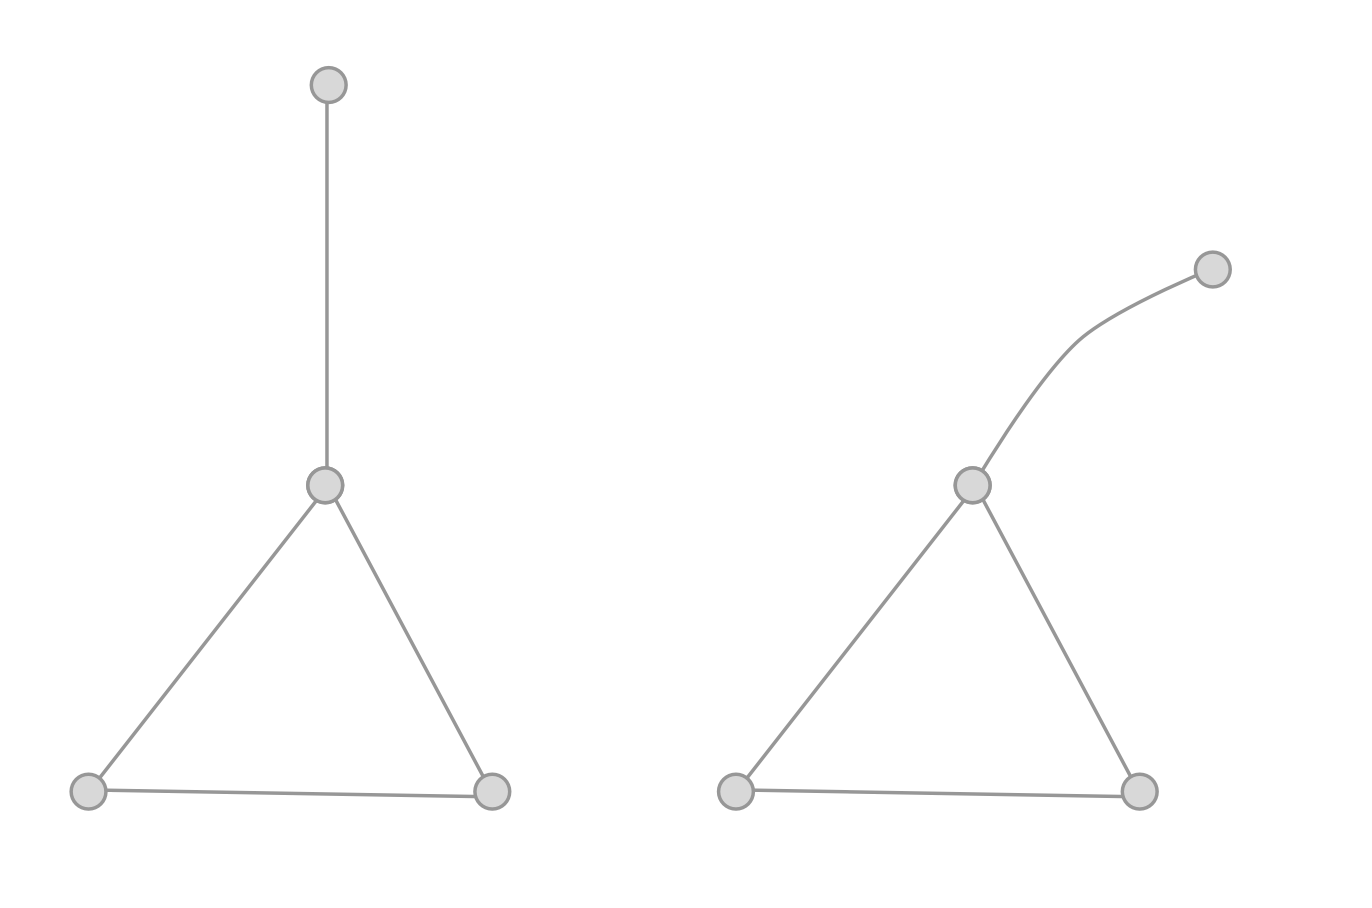
\includegraphics[height=4cm]{g2}
\end{figure}
\end{frame}



\subsection{Definició algebraica de graf}
\begin{frame}
\frametitle{Definició algebraica de graf}

\begin{block}{Definició}
Un graf $G$ es defineix com un parell ordenat de conjunts $G=(V,E) = (V(G), E(G))$ on
\begin{itemize}
\item $V$ és un conjunt no buid de punts $V=\{v_1,v_2,\cdots,v_n\}$ anomenat \textbf{vèrtexs}, i
\item $E$ és un conjunt de parells no ordenats d'elements de $V$, anomenats \textbf{arestes}
\end{itemize}
\end{block}
Si dos vèrtexs $u,v$ estan units per la mateixa aresta, aleshores direm que són \textbf{adjacents} i es representarà la seva aresta per $\{u,v\}$

En aquest cas també direm que $u$ i $v$ són \textbf{incidents} a l'aresta $\{u,v\}$

\end{frame}




\begin{frame}
\frametitle{Definició algebraica de graf}
Per representar algebraicament un graf és necessari poder distingir els vèrtexs i les arestes. Així

\begin{figure}[h]
 \label{fig:volum}
\centering
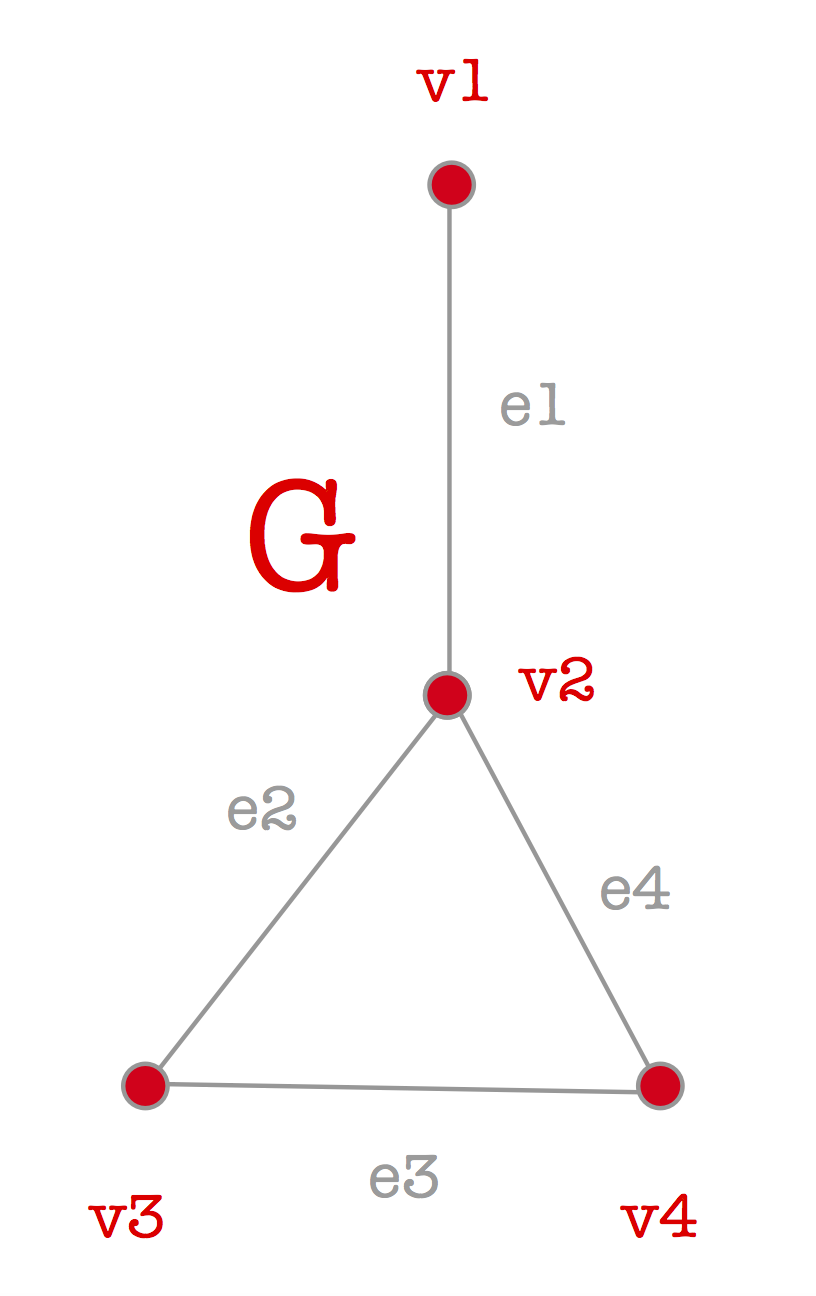
\includegraphics[height=4cm]{g3}
\end{figure}
\[G=(V(G),E(G))\]
\[V = V(G) = \{v_1,v_2,v_3,v_4\};\ \ E = E(G) = \{e_1,e_2,e_3,e_4\}\]
on $e_1 = \{v_1,v_2\}, e_2 = \{v_2,v_3\}, e_3 = \{v_3,v_4\}, e_4 = \{v_2,v_4\}$
\end{frame}









\begin{frame}
\frametitle{Definició algebraica de graf}

\begin{block}{Definicions}
\begin{itemize}
\item El nombre de vèrtexs del graf $G$, $|V(G)|$ s'anomena l'\textbf{ordre del graf}. 
\item El nombre d'arestes del graf $G$, $|E(G)|$ s'anomena la \textbf{mida del graf}.
\end{itemize}
\end{block}

\begin{block}{Graf trivial}
 Un graf $G$ és finit si $|V(G)|$ i $|E(G)|$ són finits. Si un graf finit, té un vèrtex i no té cap aresta, li direm graf trivial (correspon a un sol punt)
\end{block}
\end{frame}





\begin{frame}
\frametitle{Definició algebraica de graf}

\begin{block}{Exemple}
El següent diagrama no correspon a un graf ja que conté
\begin{figure}[h]
 \label{fig:volum}
\centering
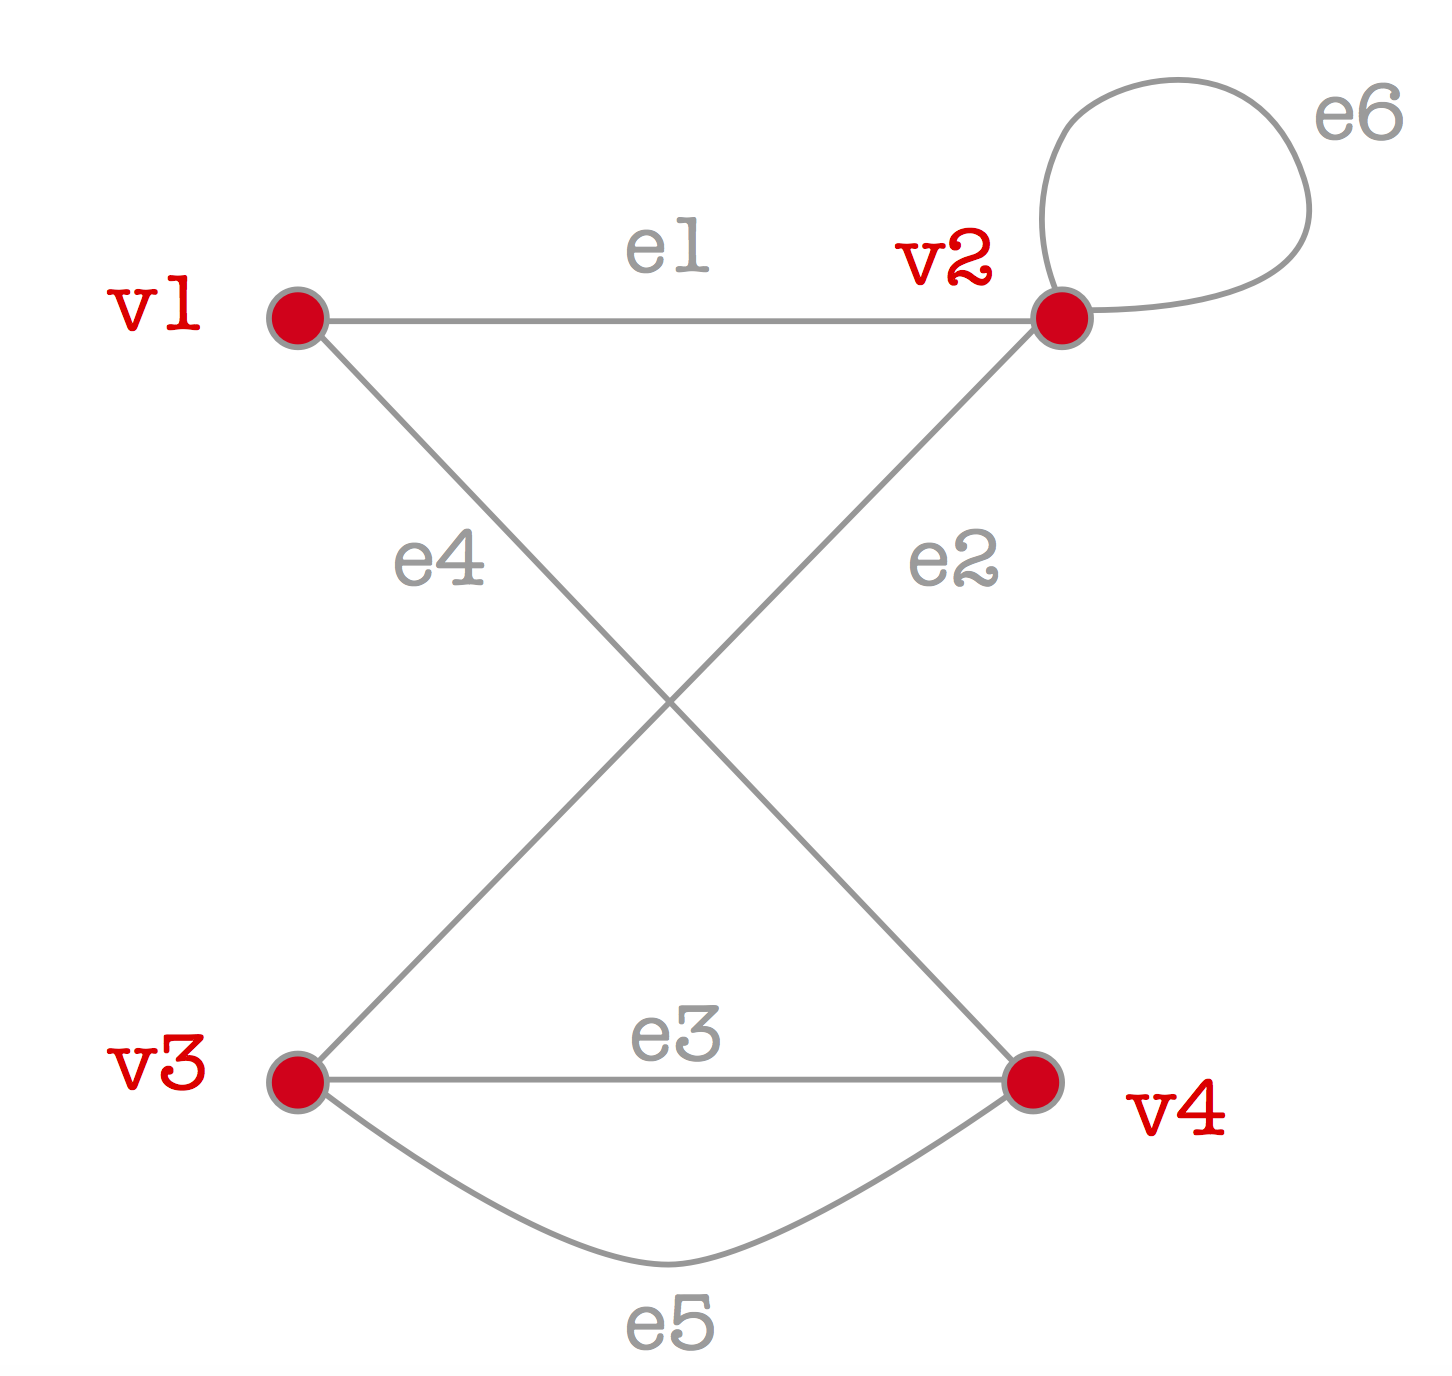
\includegraphics[height=3cm]{g4}
\end{figure}
\begin{itemize}
\item Arestes múltiples: les arestes $e_4$ i $e_5$ uneixen els vèrtexs $v_3$ i $v_4$ (multigraf).
\item Bucles: l'aresta $e_6$ uneix el vèrtex $v_2$ amb ell mateix (pseudograf). 
\end{itemize}
\end{block}
\end{frame}




\begin{frame}
\frametitle{Definició algebraica de graf}

\begin{block}{Exemple}
Notem que en aquest cas, 
\[E(G) = \{e_1=\{v_1,v_2\}, e_2=\{v_2,v_3\}, e_3 = \{v_3,v_4\}, \]
\[e_4 =  \{v_1,v_4\} , e_5 = \{v_3,v_4\}, e_6 = \{v_2,v_2\}\}\]

$E(G)$ no és un conjunt, ja que té els elements repetits $\{v_3,v_4\}$, és a dir, les arestes $e_3$ i $e_5$ i l'aresta $e_6$ comença i acaba en el mateix vèrtex. 

\end{block}
\end{frame}



\begin{frame}
\frametitle{Definició algebraica de graf}
La definició de graf donada anteriorment es correspon amb la definició que diversos autors donen de \textbf{graf simple}.  I quan es permeten arestes múltiples i/o bucles com els de l'exemple anterior, l'entenen com a \textbf{graf general}. 
\end{frame}



\begin{frame}
\frametitle{Grafs dirigits}
Un altre concepte que resulta útil és el de digraf o graf dirigit
\begin{block}{Digraf}
SIgui $G$ un graf simple (o graf general). Si a cada aresta se li assigna un sentit, direm que és un \textbf{digraf}. 

\end{block}

\begin{figure}[h]
 \label{fig:volum}
\centering
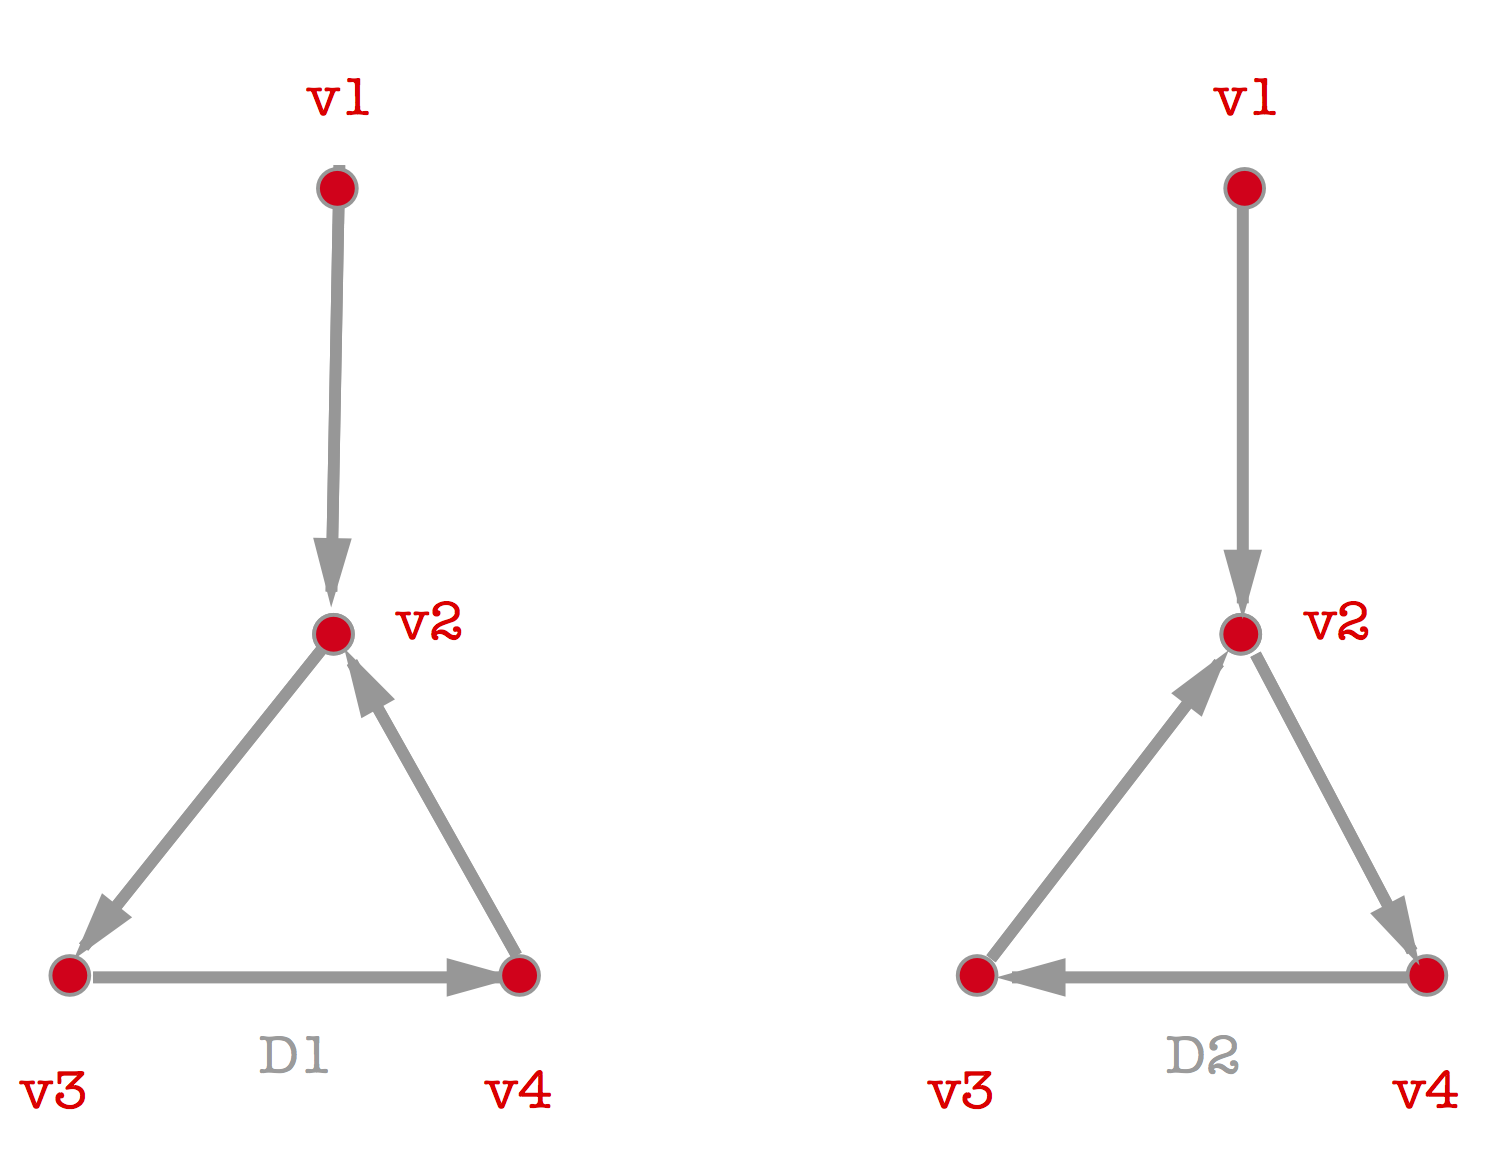
\includegraphics[height=4cm]{g5}
\end{figure}

Les arestes en aquests casos són parells ordenats $D_1\neq D_2$.

\end{frame}





\begin{frame}
\frametitle{Grau d'un vèrtex}

\begin{block}{Arestes incidents}
Direm que una aresta $e$ és \textbf{incident} amb un vèrtex $v$ si $v$ és extrem de $e$.
\end{block}

\begin{block}{Grau d'un vèrtex}

El grau d'un vèrtex $v$, $gr(v)$ és igual al nombre d'arestes que són incidents amb $v$.
\end{block}
\end{frame}




\begin{frame}
\frametitle{Grau d'un vèrtex}

Com que cada aresta és incident amb dos vèrtexos, tenim el següent resultat útil
\begin{block}{Teorema}
Sigui $G=(V,E)$ un graf, $V=\{v_1,v_2,\cdots, v_n\}$, aleshores la suma dels graus dels vèrtexs de $G$ és igual al doble del nombre d'arestes
\[\displaystyle\sum_{i=1}^n gr(v_i) = 2|E|\]
\end{block}
\end{frame}



\begin{frame}
\frametitle{Grau d'un vèrtex}

\begin{block}{Exemple}
\begin{figure}[h]
 \label{fig:volum}
\centering
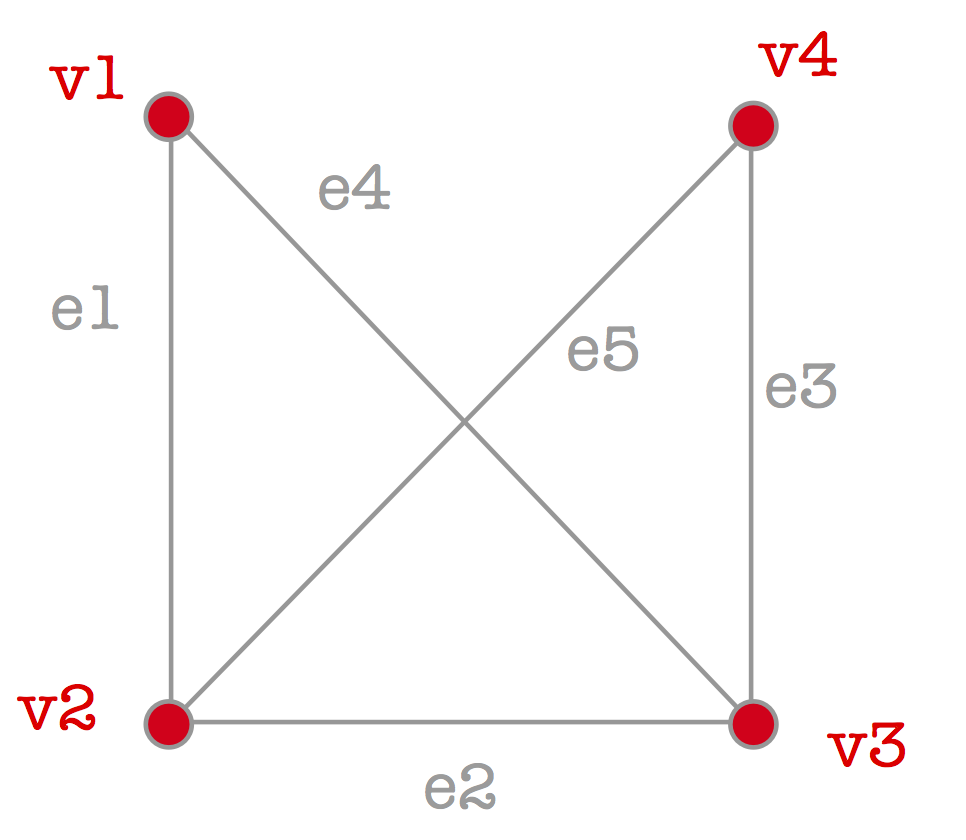
\includegraphics[height=3.5cm]{g6}
\end{figure}
\[gr(v_1) = 2\ \ gr(v_2) = 3\ \ gr(v_3) = 3\ \ gr(v_4) = 2\]
\[\displaystyle\sum_{i=1}^n gr(v_i) = 2 + 3 + 3 +2 = 10 = 2\cdot 5 =  2|E|\]
\end{block}
\end{frame}




\begin{frame}
\frametitle{Grau d'un vèrtex}

\begin{block}{Definició}
Un vèrtex és parell o imparell segons que el seu grau sigui parell o imparell.
\end{block}

\begin{block}{Teorema}
El nombre de vèrtex de grau senar d'un graf sempre és parell
\end{block}

\begin{block}{Nota}
El teorema anterior també és vàlid per a grafs generals
\end{block}
\end{frame}




\begin{frame}
\frametitle{Grau d'un vèrtex}

\begin{block}{Exemple}
\begin{figure}[h]
 \label{fig:volum}
\centering
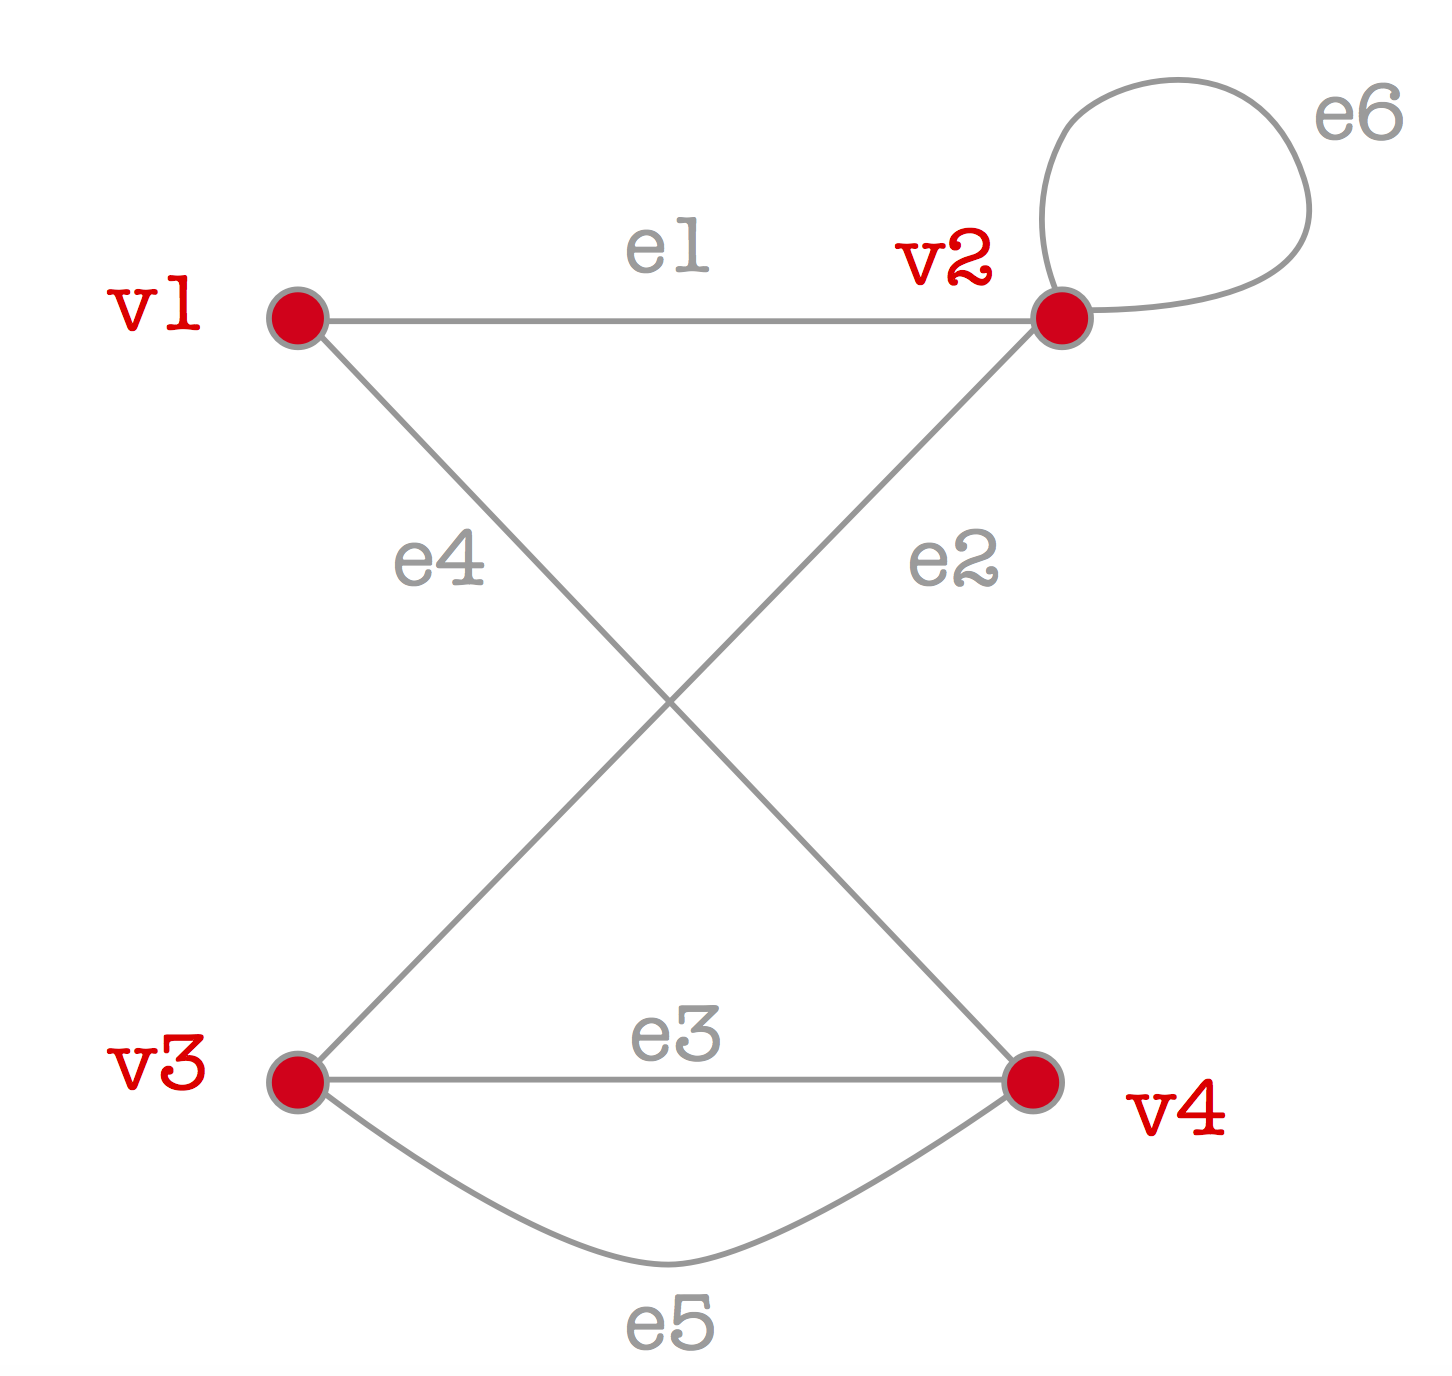
\includegraphics[height=3.5cm]{g4}
\end{figure}
\[gr(v_1) = 2\ \ gr(v_2) = 4\ \ gr(v_3) = 3\ \ gr(v_4) = 3\]
\[\displaystyle\sum_{i=1}^n gr(v_i) = 2 + 4 + 3 +3 = 12 = 2\cdot 6 =  2|E|\]
\end{block}
\end{frame}



\begin{frame}
\frametitle{Grau d'un vèrtex}

\begin{block}{Exercicis}
\begin{enumerate}
\item Dibuixau, si és possible, un graf amb 5 vèrtexs, de manera que el grau de cada vèrtex sigui 3. 
\item Dibuixau, si és possible, un graf amb 5 vèrtexs, de manera que el grau de cada vèrtex sigui 2. 
\end{enumerate}
\end{block}
\end{frame}




\begin{frame}
\frametitle{Camins}
En un graf que representi, per exemple, una xarxa de comunicacions és important conèixer l'existència de camins que recorrin totes les arestes o tots els vèrtexs i que, en certa manera, siguin els més econòmics. Per eixò veurem les següents definicions bàsiques (la nomenclatura que donam aquí no és única, hi ha autors que donen noms diferents. 
\end{frame}


\begin{frame}
\frametitle{Camins}
\begin{block}{Definició}
Un camí en un graf $G$ és una seqüència finita alternada de vèrtexs i arestes de $G$:
\[v_0\rightarrow e_1 = \{v_0,v_1\}\rightarrow v_1 \rightarrow e_2 = \{v_1,v_2\} \cdots  e_n = \{v_{n-1},v_n\}\rightarrow v_n\]
\[v_0,e_1,v_1,e_2\cdots e_n,v_n\]
on cada aresta té per extrems els vèrtexs immediataments precedent o següent de la seqüència. Per la qual cosa, el camí també pot representar-se per la seqüència de vèrtexs: $v_0,v_1,\cdots,v_n$.
\end{block}
\end{frame}



\begin{frame}
\frametitle{Camins}
\begin{block}{Extrems del camí}
Els vèrtexs $v_0$ i $v_n$ s'anomenen els extrems del camí i hom diu que el camí va de $v_0$ a $v_n$ o que connecta $v_0$ amb $v_n$.
\end{block}

\begin{block}{Longitud del camí}

La longitud del camí és el nombre d'arestes que conté. 
\end{block}
\end{frame}





\begin{frame}
\frametitle{Camins}
\begin{block}{Classificació dels camins}
\begin{itemize}
\item Recorregut: camí sense arestes repetides.
\item Camí simple: recorregut sense vèrtexs repetits excepte el primer i l'últim.
\item Camí tancat: camí en el qual els seus extrems coincideixen, és a dir, si comença i acaba en el mateix vèrtex. En cas contrari, el camí és obert. 
\item Circuit: recorregut tancat.
\item Cicle: circuit que també és camí simple
\end{itemize}
\end{block}
\end{frame}






\begin{frame}
\frametitle{Camins}
\begin{block}{Classificació dels camins}
Donat el graf classificau els següents camins
\begin{figure}[h]
 \label{fig:volum}
\centering
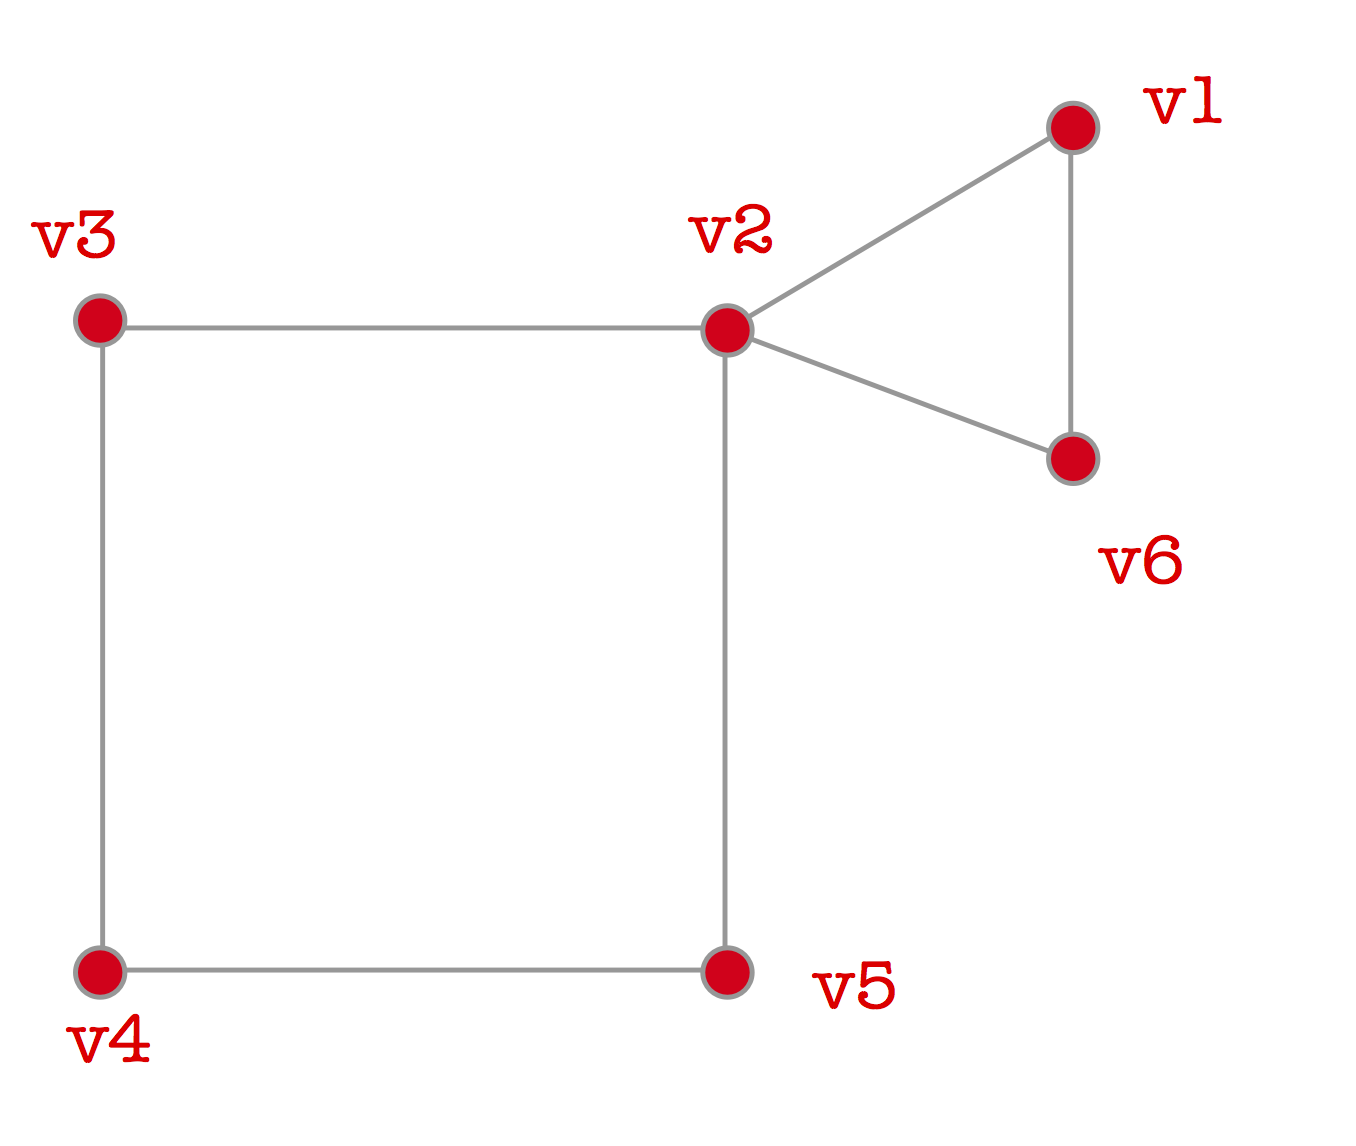
\includegraphics[height=2.5cm]{g7}
\end{figure}
\begin{itemize}
\item $v_2v_3v_4v_5v_2$
\item $v_2v_3v_4v_5$
\item $v_6v_2v_3v_4v_5v_2v_1v_6$
\item $v_1v_2v_6v_1$
\end{itemize}
\end{block}
\end{frame}





\begin{frame}
\frametitle{Connectivitat}
Existeixen grafs en els quals per a cada parell de vèrtexs $v_i,v_j$ hi  ha, almenys, un possible camí que els connecta i altres casos en els quals és impossible unir dos vèrtexs donats. 
\end{frame}


\begin{frame}
\frametitle{Connectivitat}
\begin{block}{Graf connex}
Un graf $G$ es diu que és connex si existeix un camí simple entre qualssevol parell de vèrtexs $v_i,v_j$.

En cas contrari, el graf és no connex i els vèrtexs $v_i$ i $v_j$ pertanyen a diferents components connexes del graf.

El nombre de components connexes d'un graf el notam per $K(G)$.
\end{block}
\end{frame}





\begin{frame}
\frametitle{Connectivitat}
\begin{block}{Exemple}

\begin{figure}[h]
 \label{fig:volum}
\centering
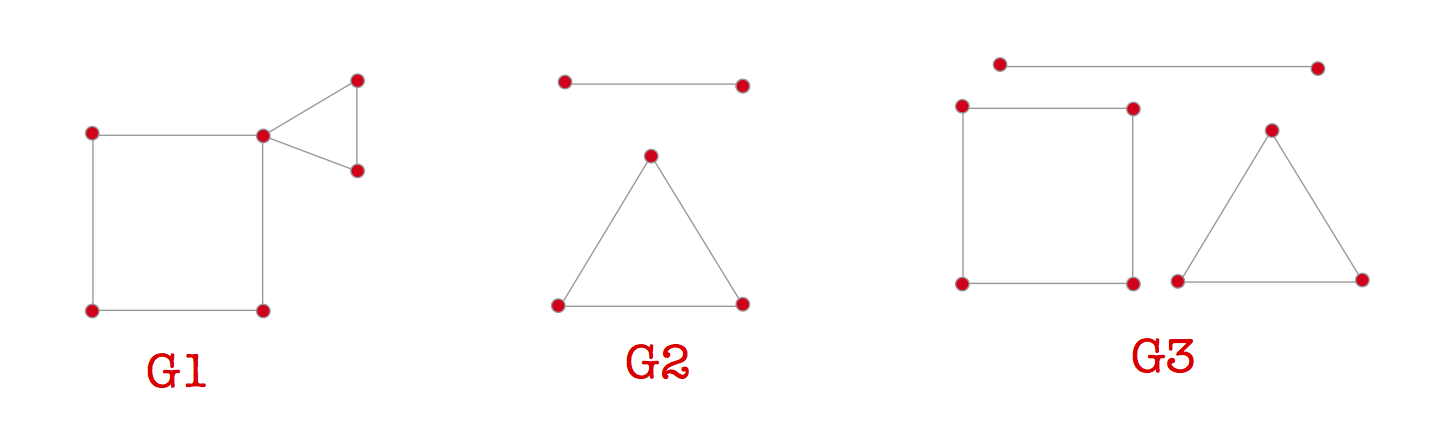
\includegraphics[height=3cm]{g8}
\end{figure}

$G_1$ és un graf connex, metres que $G_2$ i $G_3$ no ho son. $K(G_1) = 1, K(G_2) = 2, K(G_3) = 3$.
\end{block}
\end{frame}





\section{Grafs i Matrius}
\subsection{Representació matricial}

\begin{frame}
\frametitle{Representació matricial dels grafs}
\begin{block}{Definició}
Sigui $G=(V,E)$ un graf simple amb $V=\{v_1,v_2,\cdots,v_n\}$. Es defineix la seva matriu d'adjacència com  la matriu quadrada
\[A(G) = (a_{ij})_{n\times n} = \left\{\begin{array}{ll}1 & si\ v_i\ i\ v_j\ son\ adjacents \\0 & altrament\end{array}\right.\]

\end{block}
Notem que $A(G)$ és una matriu simètrica i que $a_{ii} = 0\ \forall\ i=1,\cdots,n$.

La matriu d'adjacència no és única (depèn de l'ordenació dels vèrtexs). 
\end{frame}


\begin{frame}
\frametitle{Representació matricial dels grafs}
\begin{block}{Definició}
\begin{itemize}
\item Si $G=(V,E)$ és un graf general $V=\{v_1,v_2,\cdots,v_n\}$, es defineix $A(G) = (a_{ij})_{n\times n}$ on $a_{ij}$ és el nombre d'arestes que uneixen $v_i$ amb $v_j$. Aleshores, $A(G)$ és simètrica.
\item Si $G=(V,E)$ és un digraf $V=\{v_1,v_2,\cdots,v_n\}$, es defineix $A(G) = (a_{ij})_{n\times n}$ on $a_{ij}$ és el nombre d'arestes que uneixen $v_i$ amb $v_j$. Aleshores, $A(G)$ no és simètrica.

\end{itemize}
\end{block}
\end{frame}



\begin{frame}
\frametitle{Representació matricial dels grafs}
\begin{block}{Exemple}
\begin{figure}[h]
 \label{fig:volum}
\centering
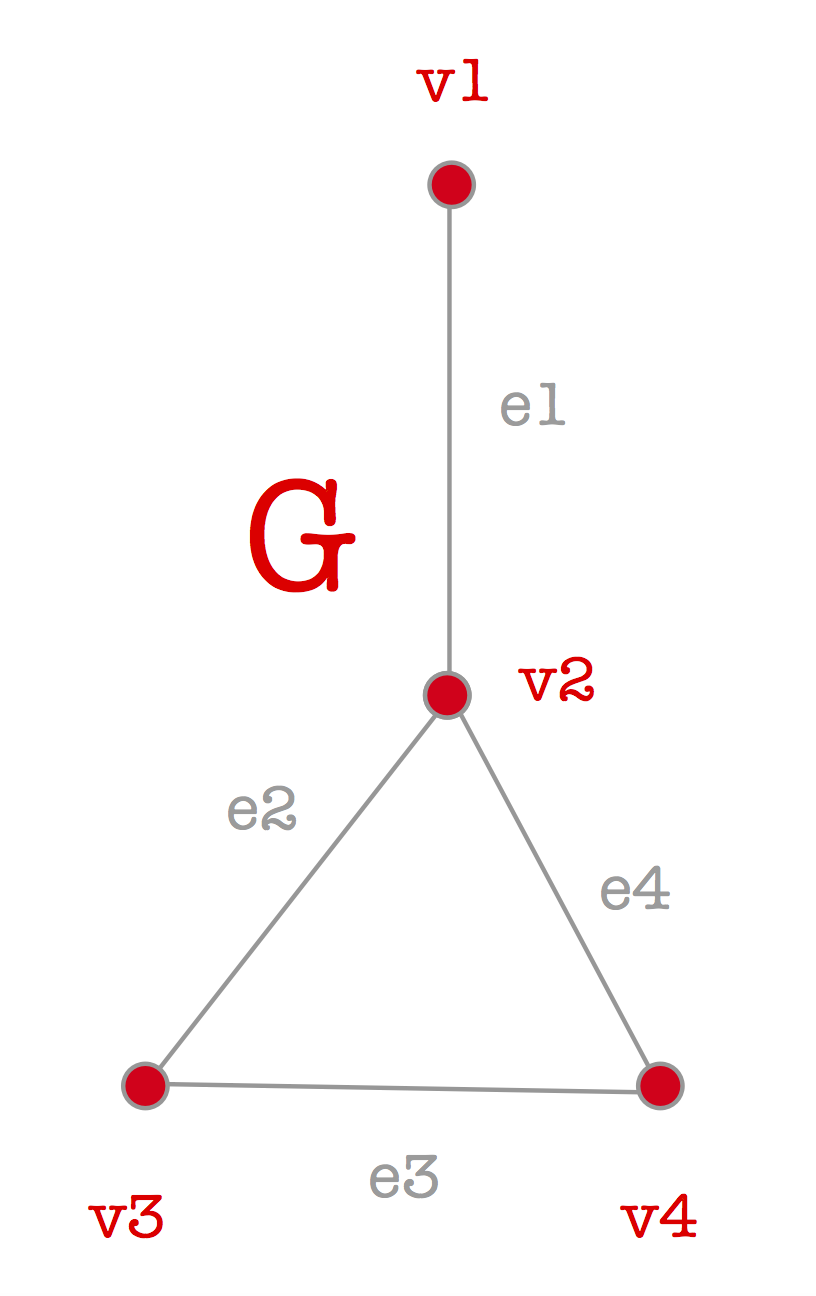
\includegraphics[height=3cm]{g3}
\end{figure}

\[A(G) = \left(\begin{array}{cccc}a_{11} & a_{12} & a_{13} & a_{14} \\a_{21} & a_{22} & a_{23} & a_{24} \\a_{31} & a_{32} & a_{33} & a_{34} \\a_{41} & a_{42} & a_{43} & a_{44}\end{array}\right) = \left(\begin{array}{cccc}0 & 1 & 0 & 0 \\1 & 0 & 1 & 1 \\0 & 1 & 0 & 1 \\0 & 1 & 1 & 0\end{array}\right)\]
Amb $a_{ij}\in\{0,1\}$ i $a_{ii} = 0$
\end{block}
\end{frame}



\begin{frame}
\frametitle{Representació matricial dels grafs}
\begin{block}{Exemple}
\begin{figure}[h]
 \label{fig:volum}
\centering
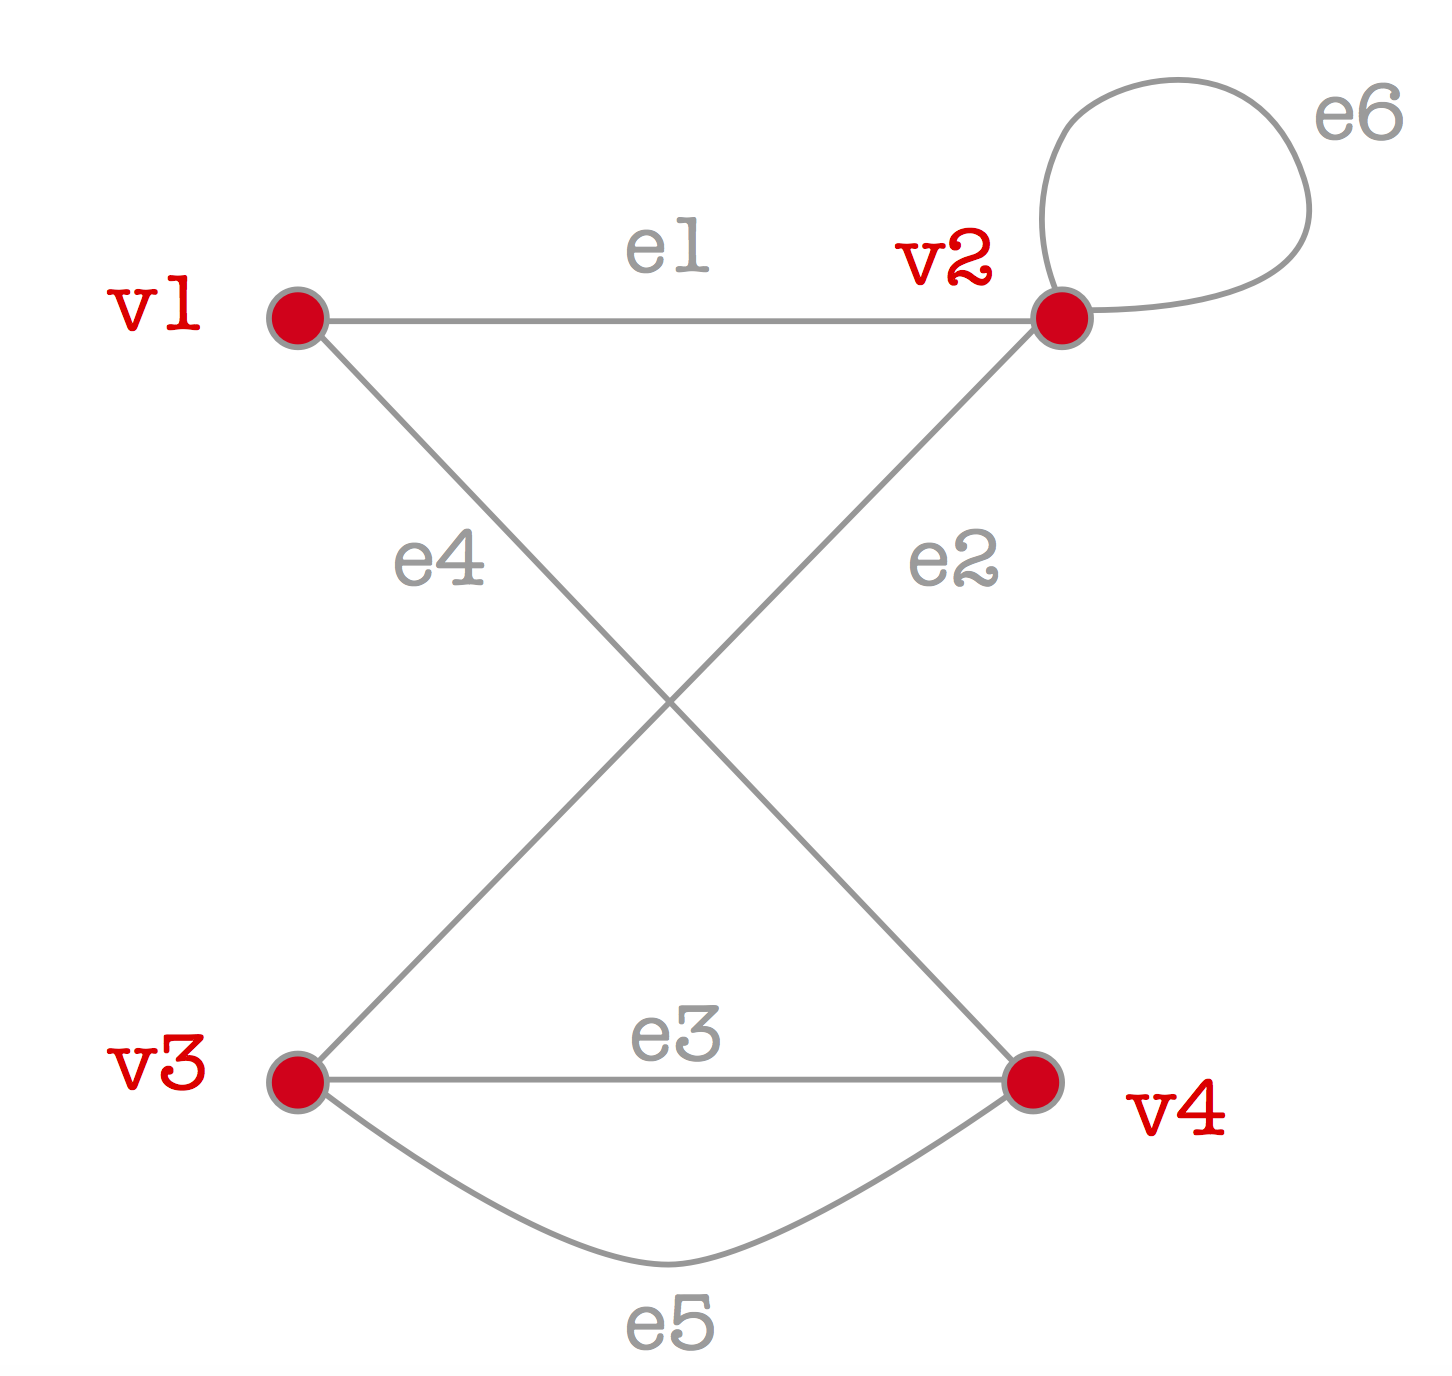
\includegraphics[height=2.5cm]{g4}
\end{figure}
\[A(G) = \left(\begin{array}{cccc}a_{11} & a_{12} & a_{13} & a_{14} \\a_{21} & a_{22} & a_{23} & a_{24} \\a_{31} & a_{32} & a_{33} & a_{34} \\a_{41} & a_{42} & a_{43} & a_{44}\end{array}\right) = \left(\begin{array}{cccc}0 & 1 & 0 & 1 \\1 & 1 & 1 & 0 \\0 & 1 & 0 & 2 \\1 & 0 & 2 & 0\end{array}\right)\]
El aquest cas $a_{ij}$ pot ser més gran que $1$ ja que el graf té arestes múltiples i $a_{ii}\neq 0$ (bucles)
\end{block}
\end{frame}






\begin{frame}
\frametitle{Representació matricial dels grafs}
\begin{block}{Teorema}
Sigue $A(G)$ la matriu d'adjacència d'un graf amb $n$ vèrtexs. Aleshores l'entrada $(i,j)$ de la matriu $A^m$ ens dóna el nombre de camins de longitud $m$ que connecten els vèrtexs $v_i$ i $v_j$.  
\end{block}
\end{frame}




\begin{frame}
\frametitle{Representació matricial dels grafs}
\begin{block}{Exemple}
Si consideram la matriu de l'exemple anterior
\[A(G) = \left(\begin{array}{cccc}a_{11} & a_{12} & a_{13} & a_{14} \\a_{21} & a_{22} & a_{23} & a_{24} \\a_{31} & a_{32} & a_{33} & a_{34} \\a_{41} & a_{42} & a_{43} & a_{44}\end{array}\right) = \left(\begin{array}{cccc}0 & 1 & 0 & 0 \\1 & 0 & 1 & 1 \\0 & 1 & 0 & 1 \\0 & 1 & 1 & 0\end{array}\right)\]
Tenim que
\[A^2(G) = \left(\begin{array}{cccc}1 & 0 & 1 & 1 \\0 & 3 & 1 & 1 \\1 & 1 & 2 & 1 \\1 & 1 & 1 & 2\end{array}\right); \ A^3(G) = \left(\begin{array}{cccc}0 & 3 & 1 & 1 \\3 & 2 & 4 & 4 \\1 & 4 & 2 & 3 \\1 & 4 & 3 & 2\end{array}\right)\]

\end{block}
\end{frame}


\begin{frame}
\frametitle{Representació matricial dels grafs}
\begin{block}{Exemple}
Considerem per exemple l'element $a_{14}$ d'aquestes tres matrius. 
\begin{itemize}
\item L'element $a_{14}$ de $A(G)$ és zero, això indica que no hi ha cap camí entre els vèrtexs $v_1$ i $v_4$, però això no indica que no es puguin connectar aquests vèrtexs. 

\item L'element $a_{14} \in A^2(G)$ prem el valor $1$, indicant així que existeix un camí de longitud $2$ que connecta $v_1$ i $v_4$. Aquest camí serà $v_1v_2v_4$.

\item L'element $a_{14}\in A^3(G)$ pren el valor $1$, aleshores existeix  un camí de longitud $3$ que connecta $v_1$ i $v_4$. Aquest camí serà $v_1v_2v_3v_4$.
\end{itemize}
\end{block}
\end{frame}

\subsection{Isomorfisme de grafs}

\begin{frame}
\frametitle{Isomorfisme de grafs}
\begin{block}{Definició}
Siguin $G(V,E)$ i $G'(V',E')$ dos grafs (o grafs generals sense bucles) i $f:V\longrightarrow V'$ una aplicació bijectiva tal que \[\{u,v\}\in E \Longleftrightarrow \{f(u),f(v)\}\in E'\]
Aleshores direm que $f$ és un isomorfisme entre $G$ i $G'$ o que $G$ i $G'$ són grafs isomorfs. 
\end{block}
En general no és fácil determinar quan dos grafs són o no són isomorfs.

Es clar que si dos grafs són isomorfs han de tenir el mateix nombre de vèrtexs i igual nombre d'arestes, però això no és suficient. 
\end{frame}

\begin{frame}
\frametitle{Isomorfisme de grafs}
\begin{block}{Teorema}
Si $G$ i $G'$ són grafs isomorfs, aleshores
\[si\ v\in V \Longrightarrow gr(v) = gr(f(v))\]
\end{block}
\end{frame}



\begin{frame}
\frametitle{Isomorfisme de grafs}
\begin{block}{Exemple}
\begin{figure}[h]
 \label{fig:volum}
\centering
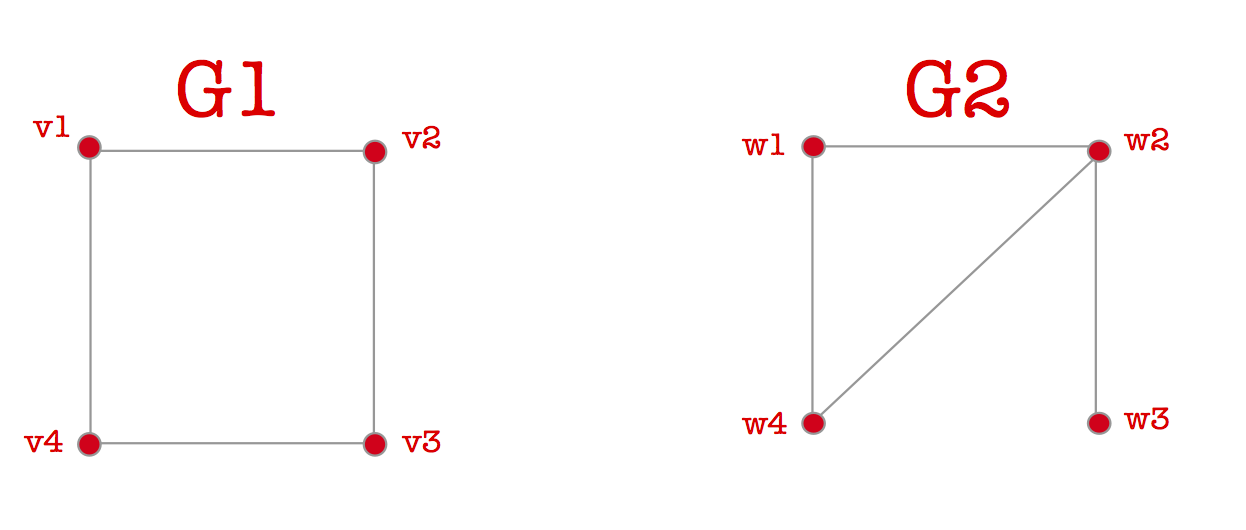
\includegraphics[height=3cm]{g9}
\end{figure}
$G$ i $G'$ tenen el mateix nombre d'arestes i el mateix nombre d'arestes.

$\forall \ v\in V(G),\ gr(v) = 2$, però en canvi $gr(w_3) = 1$, per tant $G$ i $G'$ no poden ser isomorfs. 
\end{block}
\end{frame}





\subsection{Grafs d'Euler i grafs de Hamilton}

\begin{frame}
\frametitle{Grafs d'Euler}
\begin{block}{Definició}
Sigui $G$ un graf connex
\begin{itemize}
\item Un camí eulerià és un recorregut en el qual apareixen totes les arestes. 
\item Un circuit eulerià és un camí eulerià tancat.
\item Un graf eulerià és un graf amb un circuit eulerià.
\end{itemize}
\end{block}
\end{frame}


\begin{frame}
\frametitle{Grafs d'Euler}
\begin{block}{Teorema}
Sigui $G$ un graf aleshores
\begin{itemize}
\item Si $G$ té un cirucit eulerià, el grau de cada vèrtex és  parell
\item Si $G$ té un camí eulerià, el graf $G$ té exactament dos vèrtexs de grau imparell (exactament els vèrtexs on comença i acaba el camí).
\end{itemize}
\end{block}
\end{frame}




\begin{frame}
\frametitle{Grafs d'Euler}
\begin{block}{Exemple }
Considerem el graf següent:
\begin{figure}[h]
 \label{fig:volum}
\centering
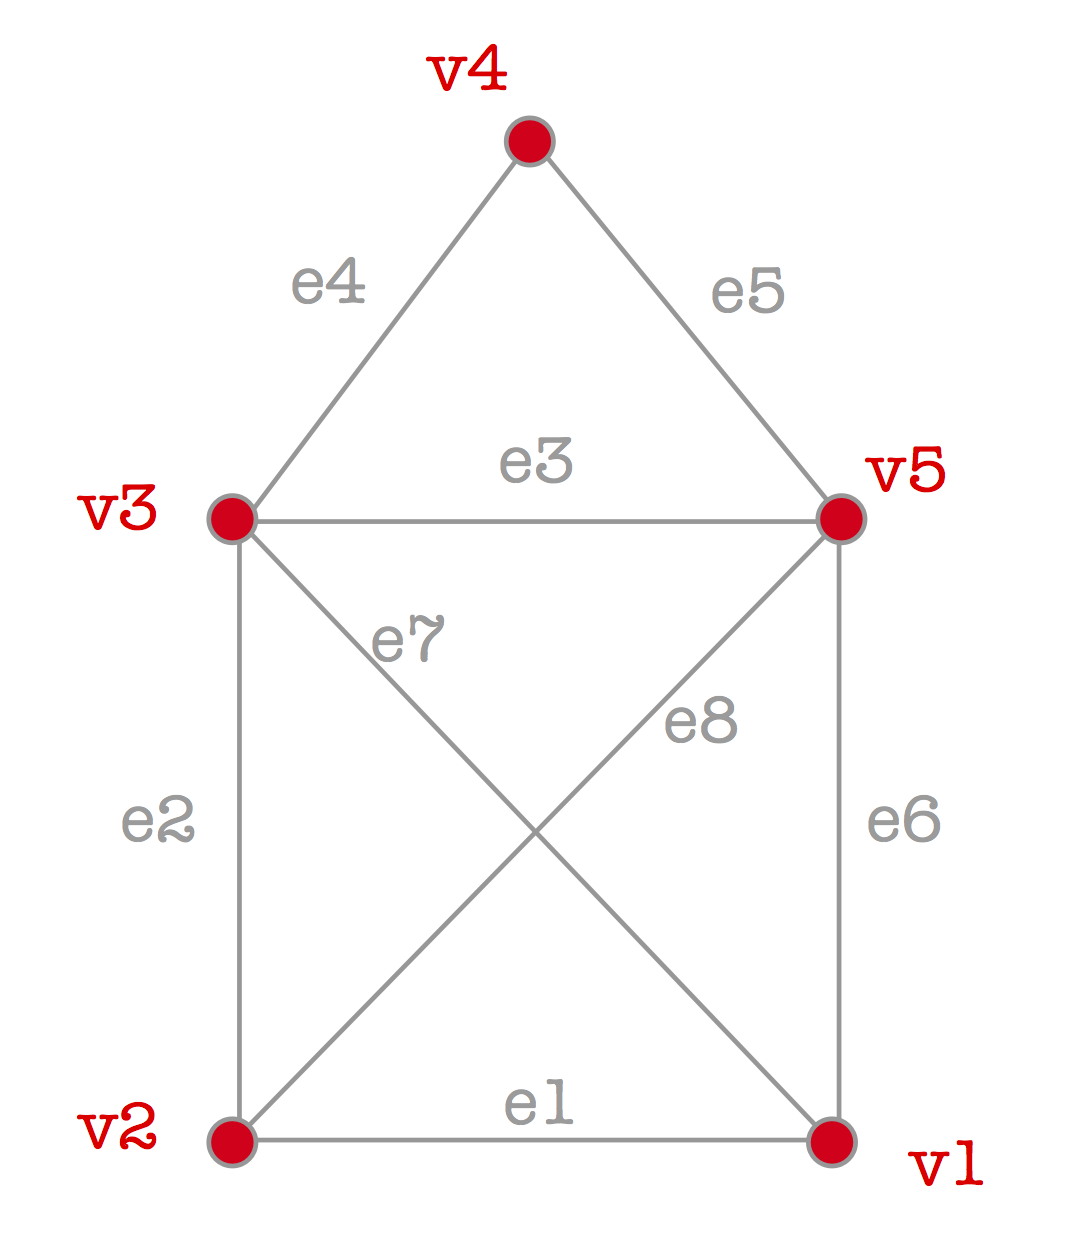
\includegraphics[height=2.5cm]{g10}
\end{figure}
La seqüencia $e_2$ $e_4$ $e_5$ $e_8$ $e_1$ $e_7$ $e_3$ $e_6$ és un camí eulerià

\[gr(v_1)=3,gr(v_2)=3,gr(v_3)=4,gr(v_4)=2,gr(v_5)=4\]

Tenim dos vèrtexs de grau 3, el camí eulerià comença en un d'ells i acaba en l'altre. 

\end{block}
\end{frame}







\begin{frame}
\frametitle{Grafs d'Euler}
\begin{block}{Exemple }
Considerem el graf que representa els ponts de Königsberg. \begin{figure}[h]
 \label{fig:volum}
\centering
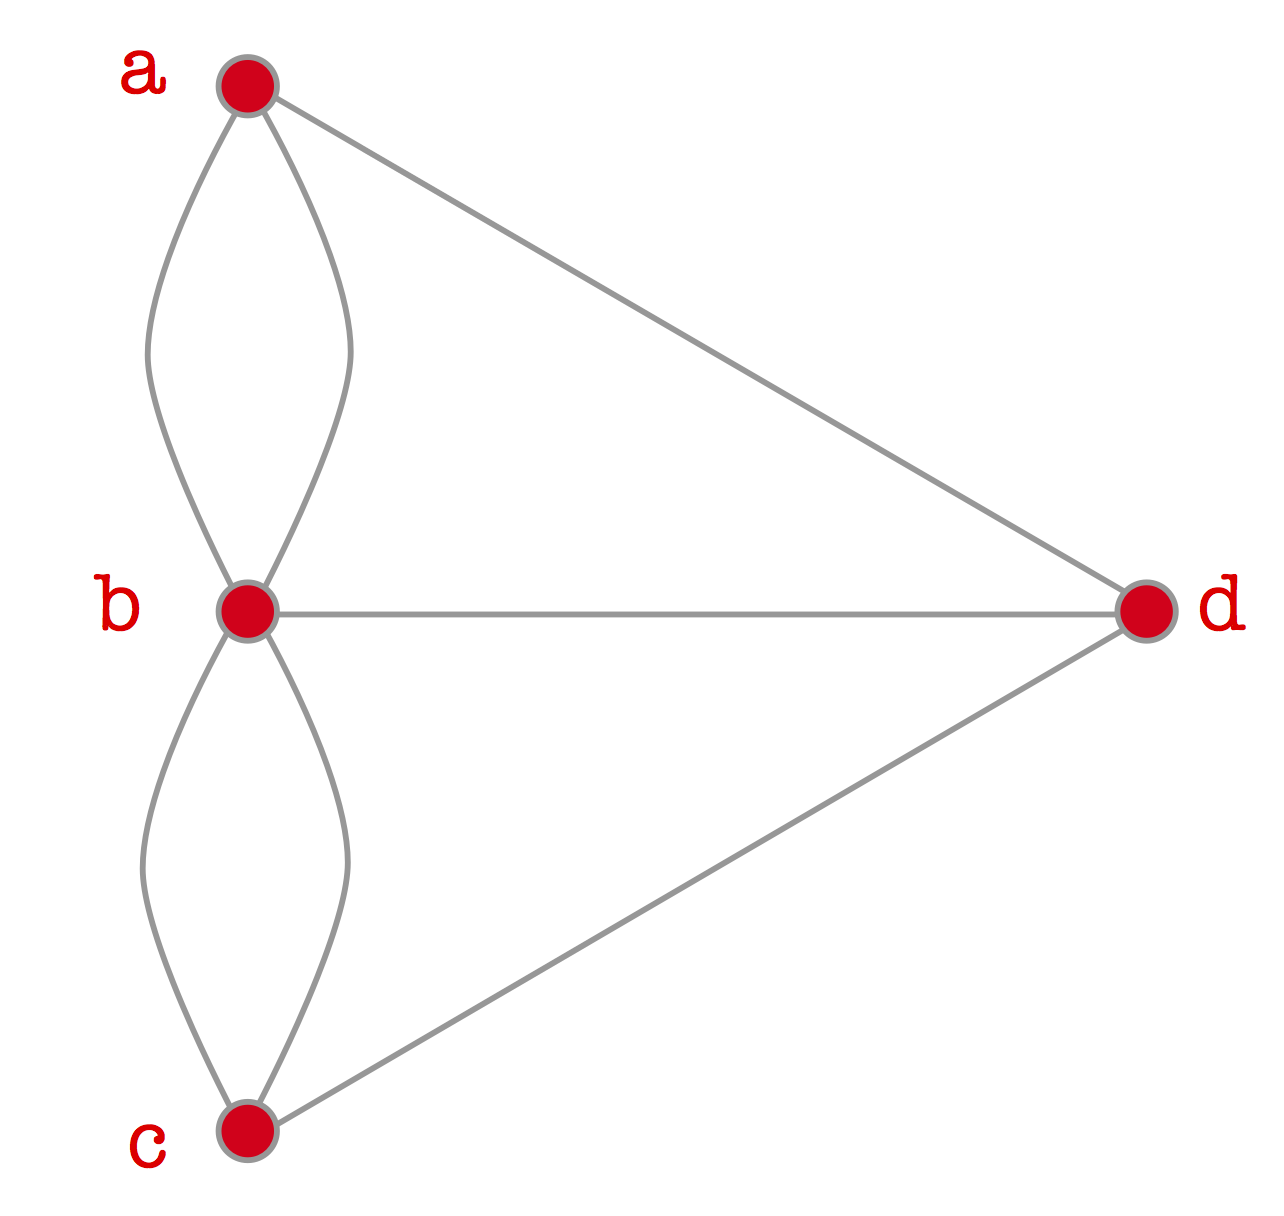
\includegraphics[height=3cm]{g11}
\end{figure}

Observam que $a,c$ i $d$ tenen grau 3 i que $b$ té grau 5. Com que tots els vèrtexs tenen grau imparell podem deduir que no existeix cap circuit eulerià. Per tant, el problema dels ponts de Königsberg no té solució. 
\end{block}
\end{frame}





\begin{frame}
\frametitle{Grafs de Hamilton}
\begin{block}{Definició }
Sigui $G$ un graf

\begin{itemize}
\item Un camí de Hamilton és un camí que recorre tots els vèrtexs només una vegada. 
\item Un circuit de Hamilton és un camí de Hamilton tancat (recorre tots els vèrtexs només una vegada tret dels extrems). 
\item Un graf amb un circuit de Hamilton s'anomena un graf de Hamilton. 
\end{itemize}
\end{block}
\end{frame}


\section{Arbres i connectivitat}

\subsection{Connectivitat}

\begin{frame}
\frametitle{Components connexes d'un graf}
Les components connexes d'un graf són els subgrafs on tots els nodes es poden connectar.

\begin{figure}[h]
\centering
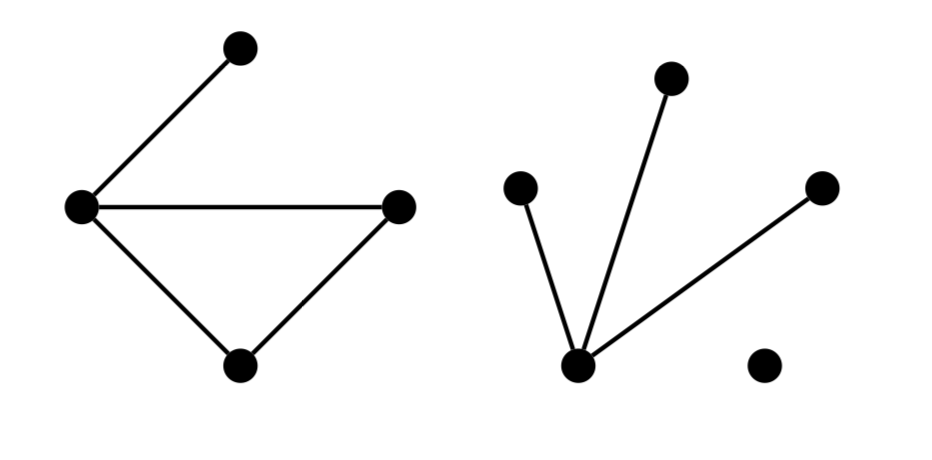
\includegraphics[height=2cm]{connex1}
\end{figure}
Un graf és connex si té una única component connexa. És a dir, si tot node és accessible desde tot node. 
\begin{block}{Proposició }
Si $G=(V,E)$ és connex, aleshores $|E|\geq |V| - 1$
\end{block}
\end{frame}

\begin{frame}
\frametitle{Arbres}
Un arbre és un graf connex sense cicles
\begin{figure}[h]
\centering
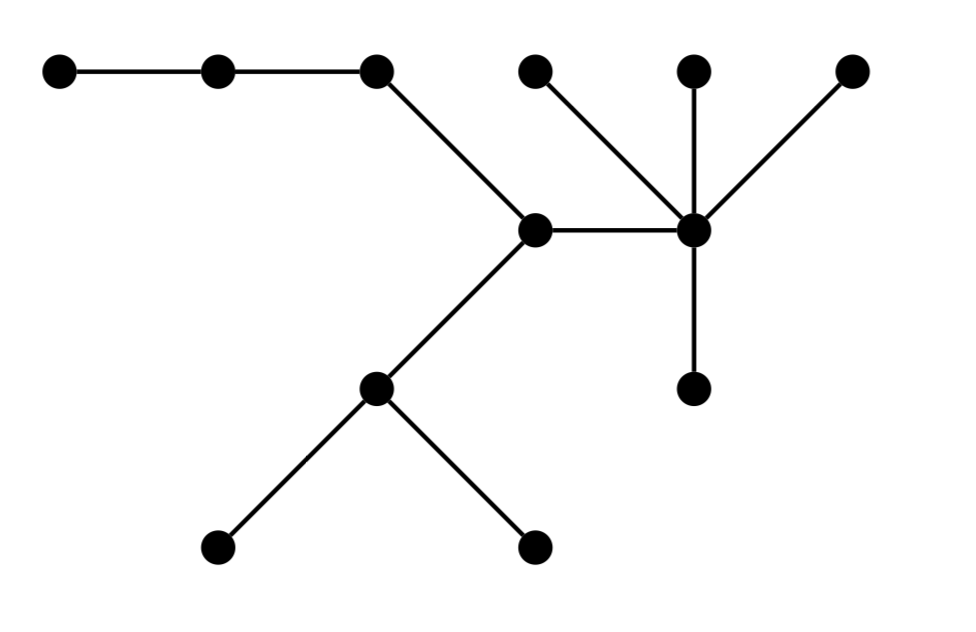
\includegraphics[height=3cm]{connex2}
\end{figure}
\end{frame}

\begin{frame}
\frametitle{Arbres}
\begin{block}{Proposició}
Sigui $G = (E,V)$ un graf, són equivalents:
\begin{enumerate}
\item $G$ és connex i sense cicles
\item Tot parell de nodes de $G$ està connectat per un únic camí
\item $G$ és connex i $|E|=|V| - 1$
\item $G$ és connex però si li treim una aresta $e\in E$ deixa de ser-ho
\item $G$ és acíclic, però si afegim una nova aresta $uv$ amb qualsevols $u,v\in V$ conté un cicle.
\end{enumerate}

\end{block}

\end{frame}


\begin{frame}
\frametitle{Arbres}
\begin{block}{Definició}
Un arbre generador d'un graf connex és un subgraf que conté tots els nodes i és, a més, un arbre. 
\end{block}
\begin{block}{Proposició}
Tot graf connex té sempre arbre generador
\end{block}
\end{frame}


\subsection{Arbre generador minimal}


\begin{frame}
\frametitle{Arbre generador minimal}
\begin{block}{Definició}
\begin{itemize}
\item Un graf amb pesos a les arestes és un graf amb funció $$w:E\rightarrow \mathbb{R}^+$$. 
\item El pes d'un subgraf és la suma dels pesos de les seves arestes. 
\item Un arbre generador minimal és un arbre generador que té pes mínim.  
\end{itemize}
\end{block}
\end{frame}



\begin{frame}
\frametitle{Algorisme de Prim}
\begin{block}{Algorisme}
Donat un graf $G=(V,E)$ amb pesos a les arestes, l'algorisme següent calcula un arbre generador minimal
\begin{enumerate}
\item Sigui $e=uv$ una aresta de pes mínim de $G$. Prenim
\[V_1 =\{u,v\};\ E_1 = \{E\};\ T=(V_1,E_1) \]
\item Per $k=2,\cdots, |V|-1$
\begin{itemize}
\item Sigui $e_k=u_kv_k$ una aresta de pes mínim tal que 
\[u_k\in V_{k-1};\ v_k\not\in V_{k-1}\]
\item Feim 
\[V_k = V_{k-1}\cup \{v_k\};\ E_k = E_{k-1}\cup \{e_k\};\ T = (V_k, E_k)\]
\end{itemize}
\end{enumerate}
\end{block}
\end{frame}

\begin{frame}
\frametitle{Algoritme de Prim - Exemple}
\begin{figure}[h]
 \label{fig:volum}
\centering
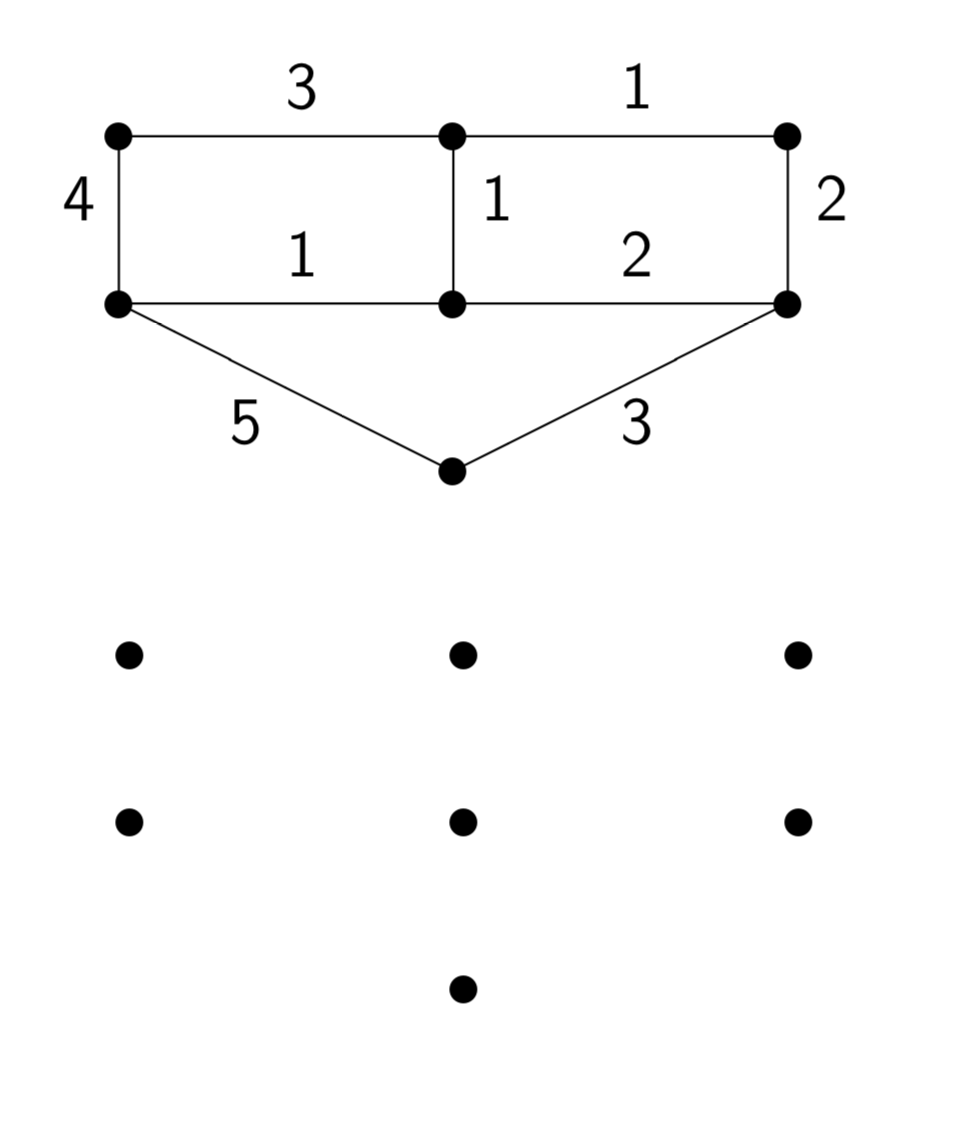
\includegraphics[height=6.5cm]{prim1}
\end{figure}
\end{frame}

\begin{frame}
\frametitle{Algoritme de Prim - Exemple}
\begin{figure}[h]
 \label{fig:volum}
\centering
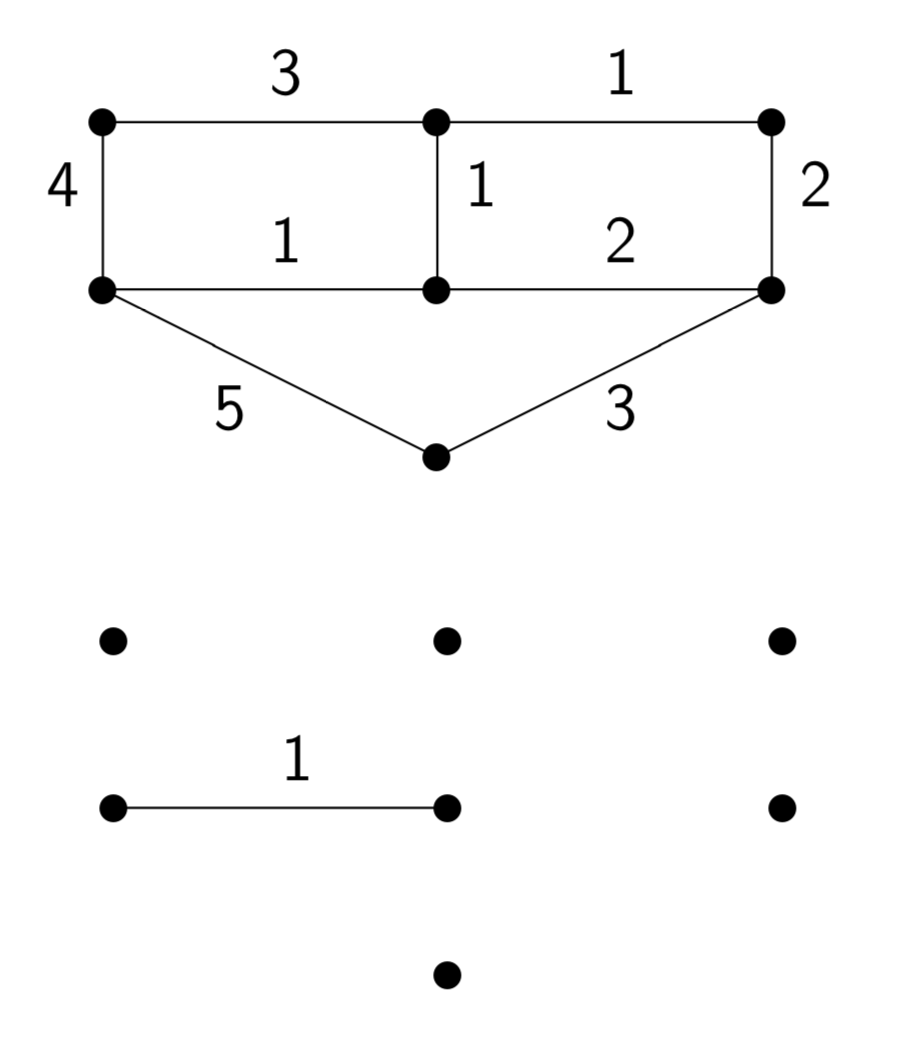
\includegraphics[height=6.5cm]{prim2}
\end{figure}
\end{frame}
\begin{frame}
\frametitle{Algoritme de Prim - Exemple}
\begin{figure}[h]
 \label{fig:volum}
\centering
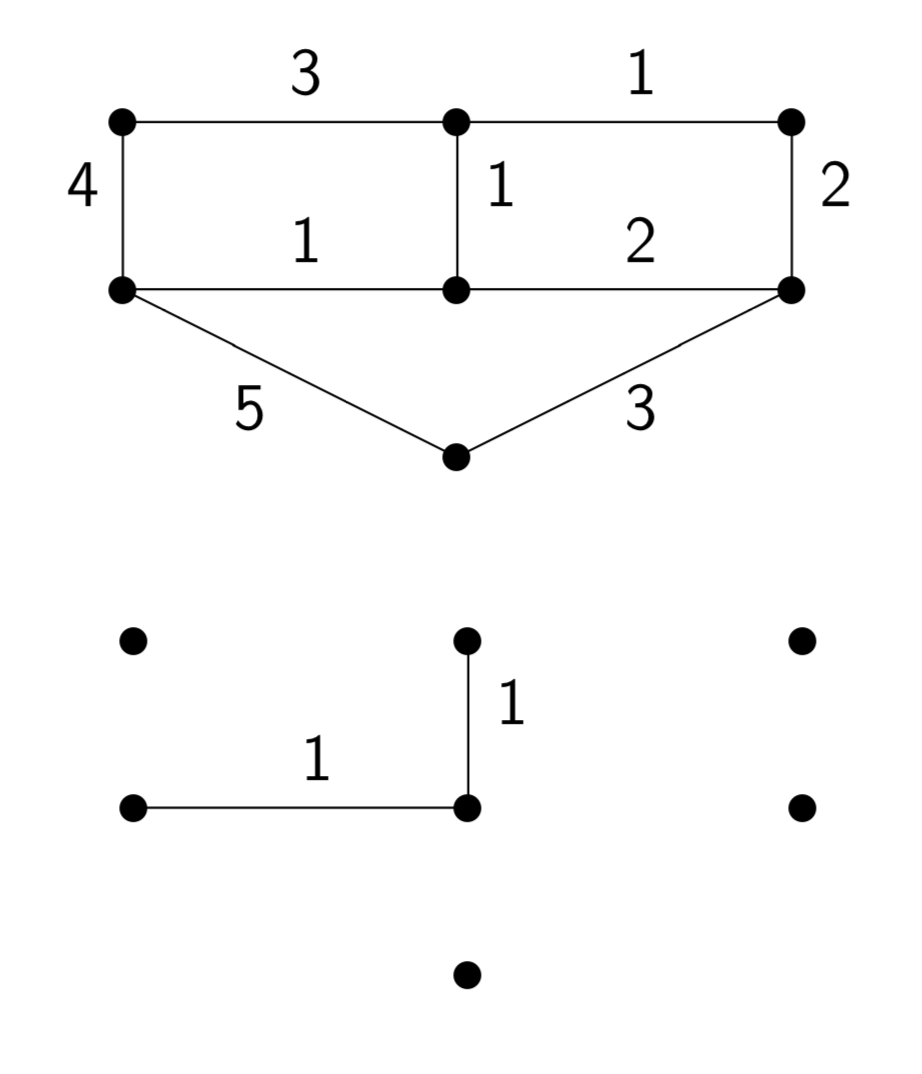
\includegraphics[height=6.5cm]{prim3}
\end{figure}
\end{frame}

\begin{frame}
\frametitle{Algoritme de Prim - Exemple}
\begin{figure}[h]
 \label{fig:volum}
\centering
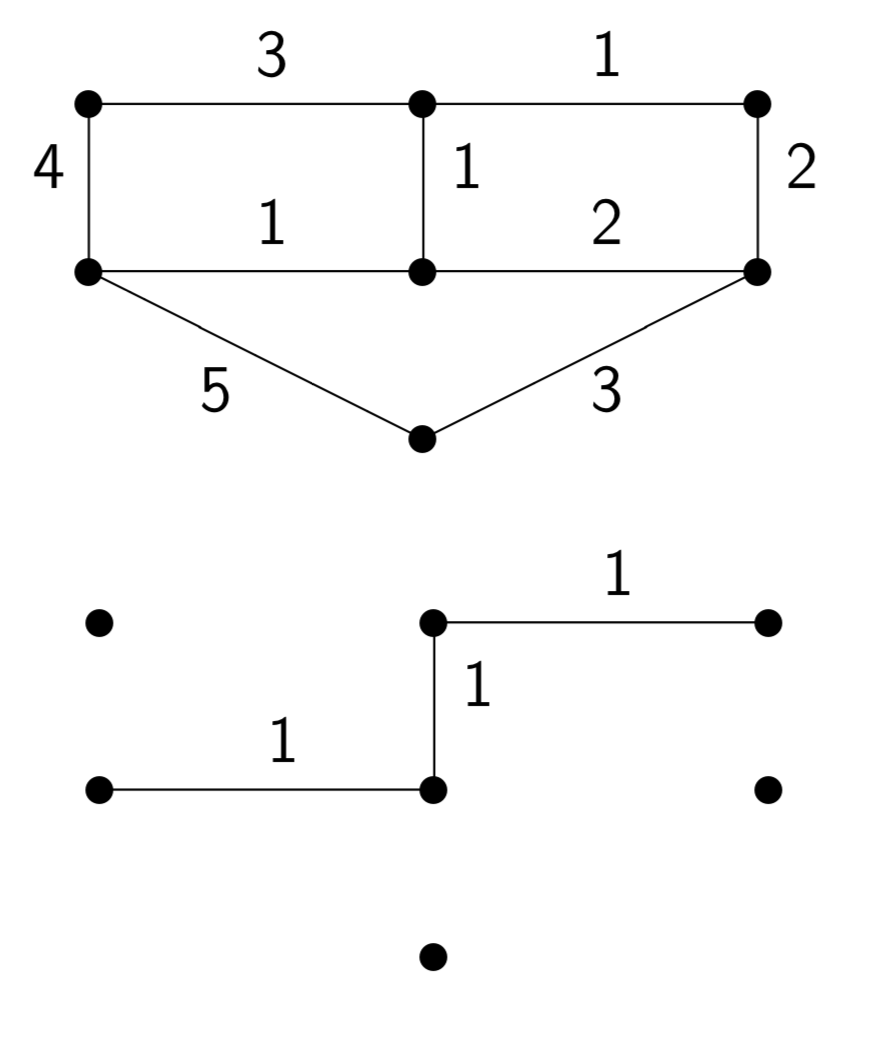
\includegraphics[height=6.5cm]{prim4}
\end{figure}
\end{frame}

\begin{frame}
\frametitle{Algoritme de Prim - Exemple}
\begin{figure}[h]
 \label{fig:volum}
\centering
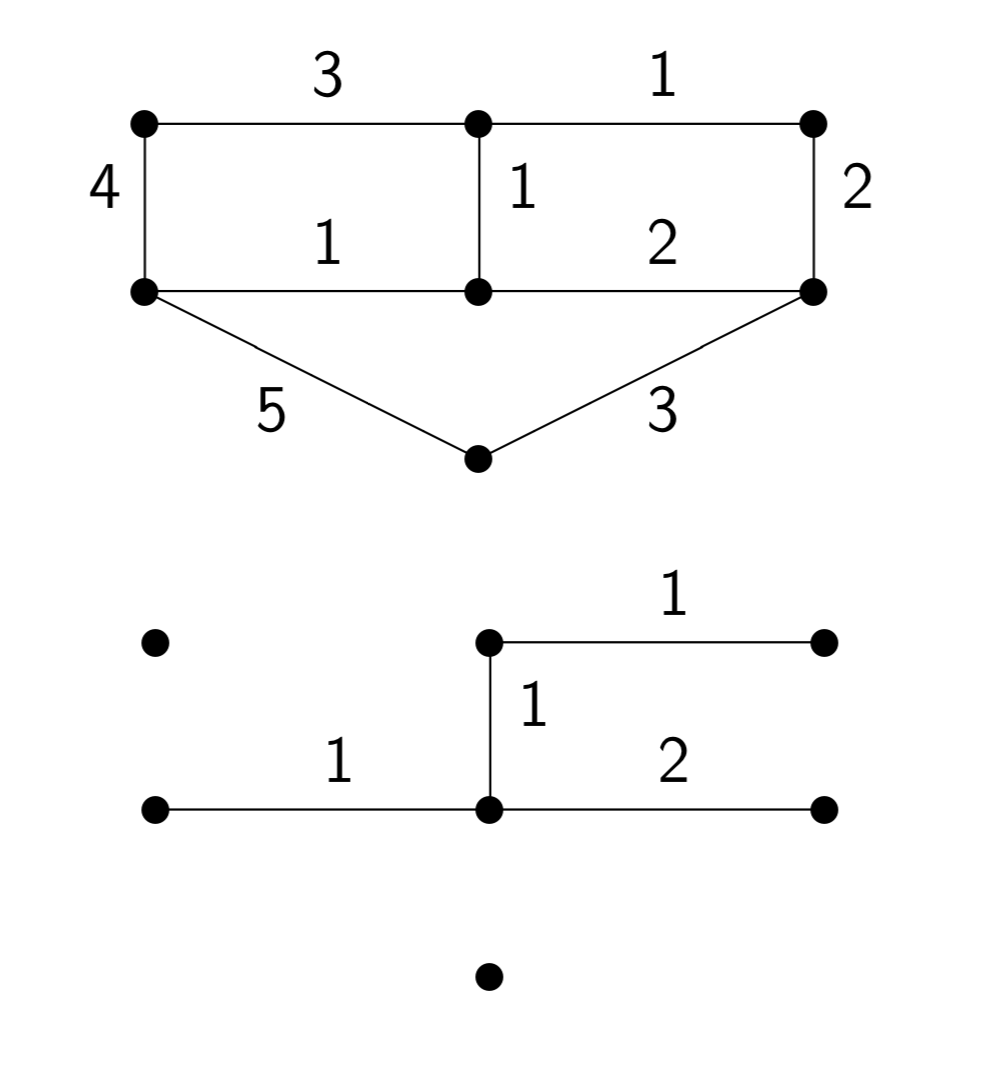
\includegraphics[height=6.5cm]{prim5}
\end{figure}
\end{frame}

\begin{frame}
\frametitle{Algoritme de Prim - Exemple}
\begin{figure}[h]
 \label{fig:volum}
\centering
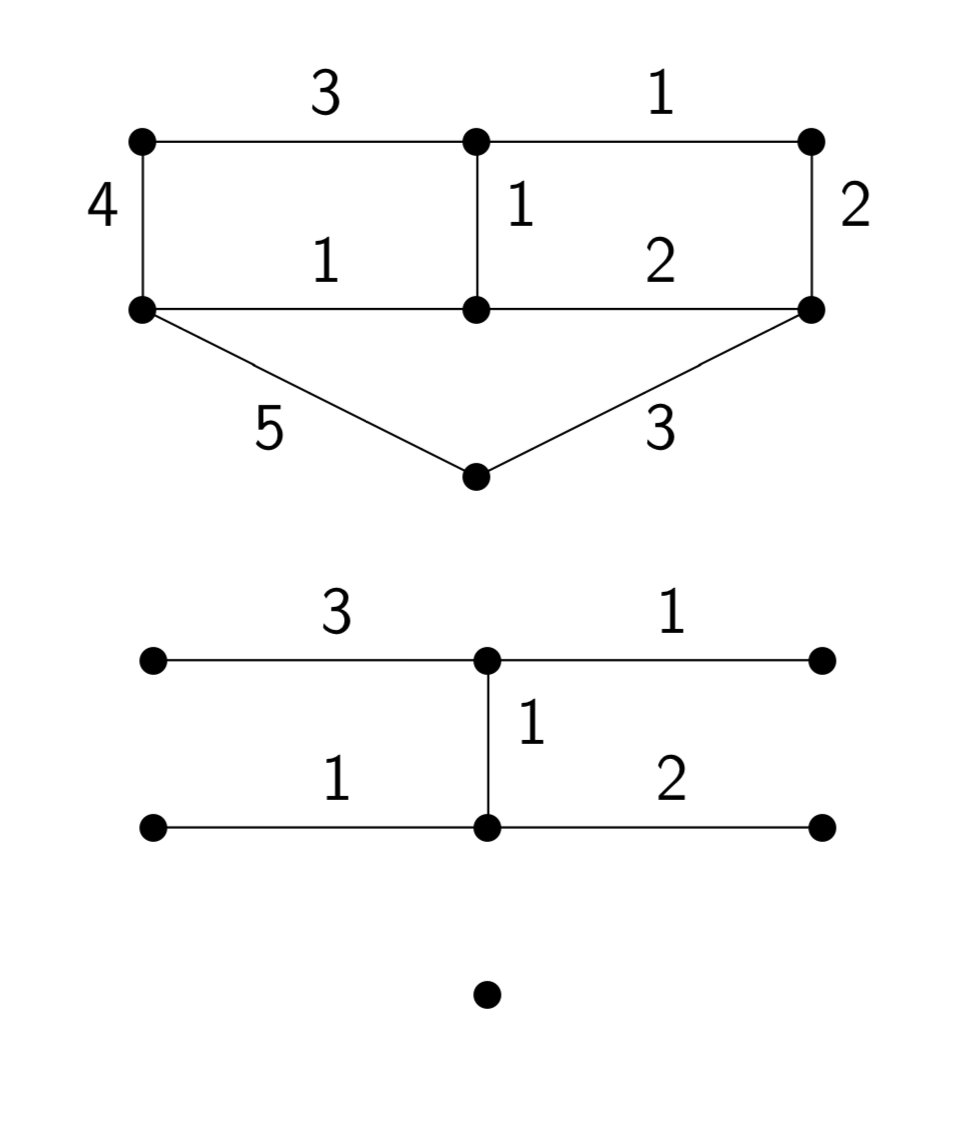
\includegraphics[height=6.5cm]{prim6}
\end{figure}
\end{frame}

\begin{frame}
\frametitle{Algoritme de Prim - Exemple}
\begin{figure}[h]
 \label{fig:volum}
\centering
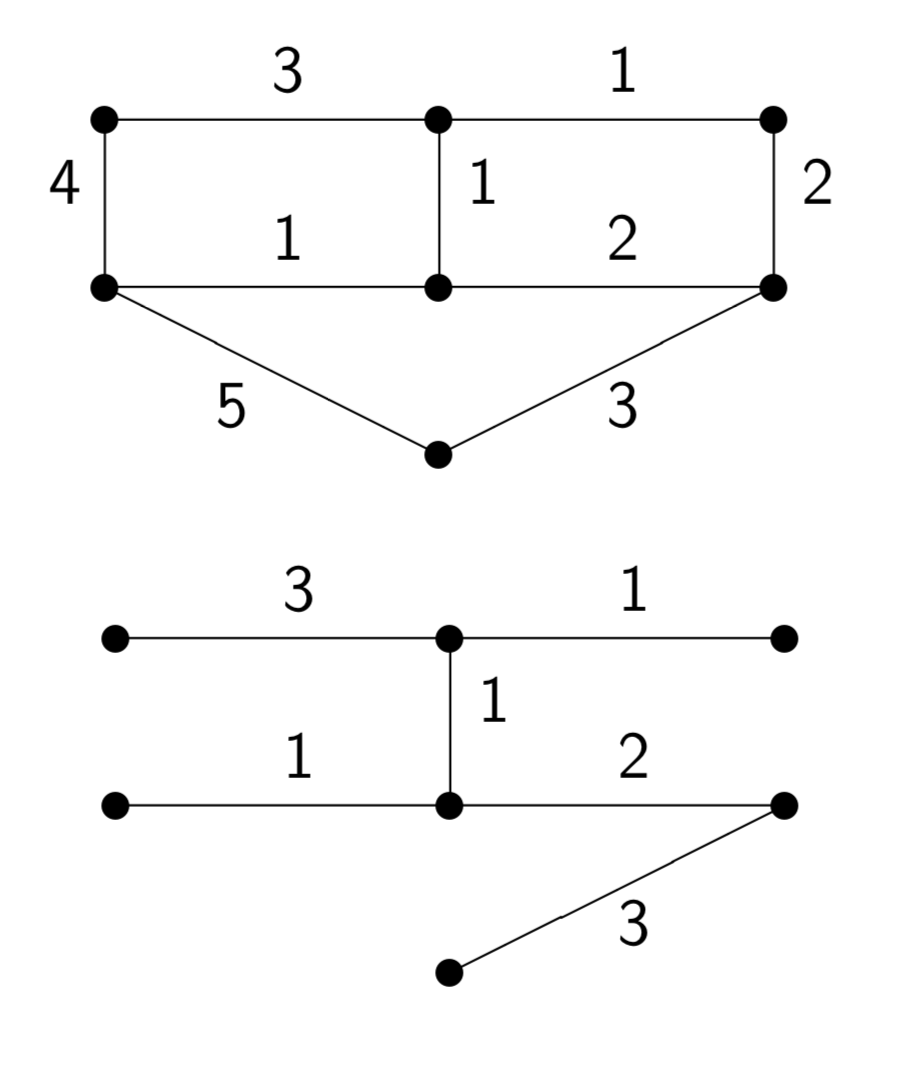
\includegraphics[height=6.5cm]{prim7}
\end{figure}
\end{frame}

\begin{frame}
\frametitle{Algoritme de Prim - Exercici}
\begin{figure}[h]
 \label{fig:volum}
\centering
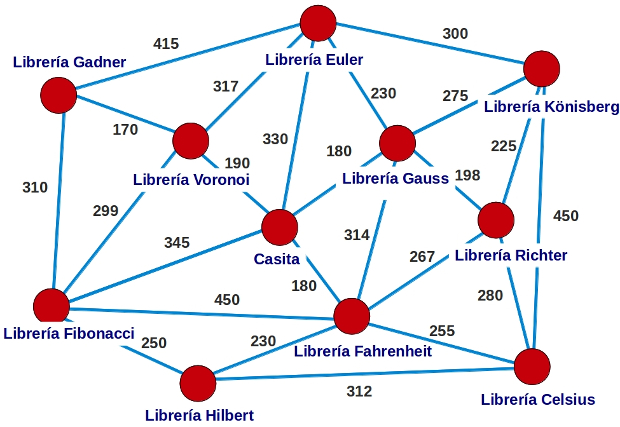
\includegraphics[height=6.5cm]{dijkstra_1}
\end{figure}
\end{frame}

\begin{frame}
\frametitle{Algoritme de Prim - Solucio}
\begin{figure}[h]
 \label{fig:volum}
\centering
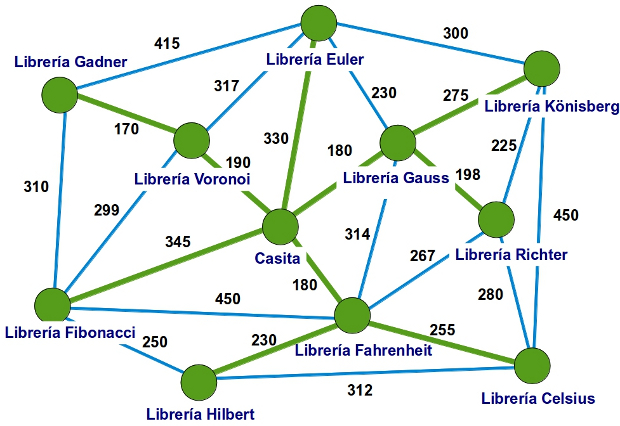
\includegraphics[height=6.5cm]{dijkstra_2}
\end{figure}

\end{frame}

%\begin{tabular}{ |p{1cm}||p{0.8cm}|p{0.8cm}|p{0.8cm}|p{0.8cm}|p{0.8cm}|p{0.8cm}|p{1.5cm}|  }
% \hline
% Z & $x_1$ & $x_2$ & $s_1$& $s_2$ & $v_1$  & $v_2$& Constants \\
% \hline
%1 &0 & 130 & -100 & 33& 0& -133 & 404 \\
%0 & 0 &  4/3 & -1 & 1/3 & 1 & -1/3 & 4 \\
%0 & 1 & 2/3 & 0 & -1/3 & 0 & 1/3  & 4 \\
% \hline
%\end{tabular}
%\end{frame}


%  \begin{figure}[h]
  %  \label{fig:volum}
%\centering
%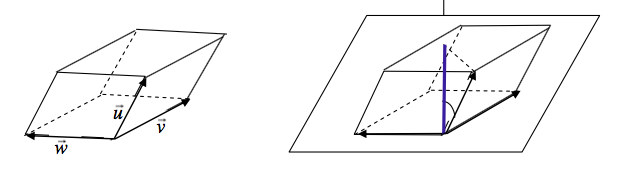
\includegraphics[height=3cm]{volum}
%\end{figure}


\end{document}